\documentclass{article}
\usepackage{fontspec}
\usepackage{polyglossia}
\setdefaultlanguage{french}
\usepackage[a4paper,margin=2.25cm]{geometry}

\usepackage{amsmath}
\usepackage{array}
\usepackage{auto-pst-pdf}
\usepackage{booktabs}
\usepackage{cite}
\usepackage{graphicx}
\usepackage{lmodern}
\usepackage{marvosym}
\usepackage{mathrsfs}
\usepackage{minted}
\usepackage{multicol}
\usepackage{multirow}
\usepackage{paralist}
\usepackage{schemabloc}
\usepackage{siunitx}
\usepackage{soul}
\usepackage{tikz}
\usepackage[european,cuteinductors,siunitx]{circuitikz}
\usepackage{url,hyperref}
\usepackage{verbatim}
\usepackage{xunicode,xltxtra}

\title{
\includegraphics{../../images/inp-enseeiht} \\ ~ \\ ~ \\ ~ \\ ~ \\ Rapport de stage de seconde année \\ ~ \\ ~ \\ 
\includegraphics[width=\linewidth]{img/swir.jpg} \\ ~ \\}
\author{Guilhem Saurel}
\date{\oldstylenums{\today}}

\begin{document}

\begin{titlepage}
    \setcounter{page}{0}
    \maketitle
    \thispagestyle{empty}
\end{titlepage}

\tableofcontents
\setcounter{page}{0}
\thispagestyle{empty}

\clearpage

\section{Présentation de l’entreprise}
\subsection{Histoire et position actuelle}

L’entreprise toulousaine Anyware Technologies, rachetée en février 2008 par Wave Com, a fusionné avec Sierra Wireless en avril 2009.

Sierra wireless est une entreprise internationnale positionnée sur les secteurs des télécomunnications sans fil (comme son nom peut le laisser présager) et plus récement du M2M et de l’IoT.

\begin{figure}[h!]
    \centering
\includegraphics[width=\linewidth/2]{img/anyware-tech.png}
    \caption{Anyware Technologies}
\end{figure}

~

Son siège social se situe à Richmond, au Canada, mais elle dispose également de bureaux en Californie, en République Populaire de Chine (Guangdong \& HongKong), et bien sûr en France (Paris \& Labège). C’est dans ce bureau de Labège que j’ai effectué mon stage, parmis les anciens d’Anyware Technologies et de Wave Com, mais également des ingénieurs, managers et commerciaux de Sierra Wireless provenant du monde entier, régulièrement de passage ou même installés sur le site.

\begin{figure}[h!]
    \centering
\includegraphics[width=\linewidth/2]{img/swir.jpg}
    \caption{Sierra Wireless: http://www.sierrawireless.com/}
\end{figure}

\subsection{Compétences et produits}

Ce bureau Toulousain est baptisé «Solutions \& Services», et s’occupe donc principalement de développement logiciel, firmware et web, ainsi que de l’adminstration système ; mais Sierra Wireless est surtout connue pour sa conception et sa fabrication de modems sans fil 2G, 3G et 4G, de routeurs, de passerelles, et de modules M2M.

~

Ses produits sont disponibles soit à travers ceux de certains OEMs soit directement via des revendeurs, et visent un grand nombre d’applications telles que les automobiles et les transports, les services publics, la santée, la sécurité, les énergies, les infrastructures industrielles, les ordinateurs et téléphones portables, et les réseaux.

Parmis ces produits, on peut citer trois principales gammes:

\begin{description}
    \item[AirLink] Routeurs et passerelles embarqués,
    \item[AirPrime] Modules programmables apportant des connectivités 2G, 3G et 4G, en PCI-Express ou SMD, à des téléphones, tablettes, et ordinateurs portables,
    \item[AirVantage] Plateforme Cloud servant à gérer des flottes de produits AirLink et AirPrime, depuis l’interface web ou des APIs.
\end{description}

\clearpage

\section{Sujet, débuts et premières impressions du stage}
\subsection{Sujet du stage}

Depuis peu, la stratégie de Sierra Wireless est passée du côté lumineux de la force en intégrant des composantes entièrement open source à son catalogue, afin d’attirer l’attention de plus de développeurs.

Dans ce cadre, Benjamin Cabé, «Open Source M2M Evangelist» chez Sierra Wireless Solutions \& Services, a eu l’idée de profiter de l’incroyable notoriétée de la Raspberry Pi en proposant un shield 3G Sierra Wireless, et éventuellement un module GPS.

~

Lorsque je me suis présenté à la recherche d’un stage, il m’a donc proposé de développer les interfaces logicielles nécessaires à un tel matériel, ainsi que d’en faire la promotion en proposant une application utile, qui pourrait être présentée sur le blog officiel de la fondation Raspberry Pi. Quelques semaines plus tard, j’ai appris que l’idée du module GPS avait été abandonnée, et qu’il y avait des difficultées pour la conception du shield.

\subsection{Débuts du stage}

Enfin, mon année scolaire terminée, lorsque j’ai commencé mon stage mi-juin, j’ai appris que le shield n’était toujours pas prêt, et j’ai donc proposé mes compétences pour le faire moi-même. Disposant des plans de cartes similaires open-source, de mon expérience en routage accumulée à l’INP-ENSEEIHT, lors de mon stage à l’ULB et au club robotique de l’école, ainsi que de mes connaissances en routage d’antennes du projet Hyper-Fréquences, je pensais être capable d’y parvenir, mais je n’étais pas capable d’assurer un délai de réalisation compris dans la durée de mon stage de 9 semaines.

~

Après un certain moment de discussion, d’hésitation, et quelques rendez-vous, il a été décidé que l’entreprise Toulousaine Snootlab s’occuperait finalement de la conception de cette carte, vu qu’elle venait de recruter un nouvel ingénieur, et que ce serait donc sa première mission de test.

\begin{figure}[h!]
    \centering
\includegraphics[width=\linewidth/2]{img/snoot.jpg}
    \caption{Snootlab: http://snootlab.com/}
\end{figure}

Le lancement étant prévu pour septembre, il n’était donc plus envisageable que je puisse aider à quoi que ce soit sur ce sujet ; mais heureusement, un grand nombre d’autres activités m’ont été proposées, ce qui m’a permis d’en essayer diverses, dans un cadre particulièrement différent de ce que j’avais pu connaître dans une PME ou dans un laboratoire de recherche.

\subsection{Premières impressions sur le stage}

Parmis les choses qui m’ont vraiment plu dans cette entreprise, on peut compter
les «Make-it», une journée toute les trois semaines que chaque employé peut prendre pour réaliser n’importe quel projet qui le tient à cœur (sous résèrve de le présenter aux autres lors d’une réunion),
une impressionnante collection de jouets électroniques (voir l’Annexe A pour une liste non-exhaustive),
un Comité d’Entreprise donnant notamment accès à une clef illimitée pour la machine à boissons chaudes,
certaines réunions où il était question de stratégie industrielle à l’échelle internationnale sur plusieurs années,
le cadre agréable et la proximitée du lac de Labège alors qu’on n’est qu’à trois quarts d’heure de transports de l’école ou de chez moi,
la bonne humeur, l’expertise technique et la créativité de la plupart de mes collègues,
ou encore la flexibilité horaire laissée aux employés (et stagiaires).

~

Naturellement, on peut aussi compter certains désagréments, mais pour ma part, mon principal problème aura été d’avoir dilapidé la majorité de mon salaire, pourtant plutôt bon, dans les différents restaurants de Labège le midi, tous plus attirants les uns que les autres. Mais je ne peux bien sûr m’en prendre qu’à ma gourmandise.

\clearpage

\section{Création de paquets pour diverses distributions logicielles et diverses architectures matérielles}
\subsection{Mihini}

Sierra Wireless propose une architecture réseau allant de ses modems, routeurs et passerelles vers son application Cloud: Airvantage.
Pour cela, la communication s’effectue selon un protocole de communication maison: le M3DA (http://wiki.eclipse.org/images/d/d4/M3DAProtocolSpecification.pdf).

~

Ce protocole étant peu répandu hors de Sierra Wireless, l’idée est apparue de créer un logiciel léger, et donc capable de fonctionner même sur des systèmes embarqués peu puissants et à faible consommation, qui utiliserait ce protocole et AirVantage, comme si c’était un produit AirLink ou AirPrime, afin d’exposer une API LUA pour permettre la création d’applications M2M.

~

Ainsi est né Mihini, un projet open-source hébergé par la fondation Eclipse, et donc l’un des trois piliers de la partie M2M de la fondation Eclipse

\begin{figure}[h!]
    \centering
    
\includegraphics{img/mihini_logo.png}
    
\includegraphics[width=\linewidth/3]{img/M2M.png}
    
\includegraphics{img/eclipse.png}
    \caption{Mihini: http://www.eclipse.org/mihini/, M2M Eclipse: http://m2m.eclipse.org/, et Eclipse.}
\end{figure}

\subsection{Empaquettage}
Cet outil, particulièrement pratique car on peut utiliser des comptes d’essai d’AirVantage, mais aussi un serveur open source M3DA (https://github.com/SierraWireless/m3da-server), commence à être apprécié et utilisé par la communeauté, mais il était relativement long et difficile à installer.

~

J’ai ainsi réalisé des paquets à l’aide de CPack pour les distributions Debian et dérivées (.deb), celles de Red Hat (.rpm) et les autres (.tar.gz), et pour les architectures processeur i386, amd64, armhf et armel. J’ai également ajouté des scripts d’installations, de mise à jour et de désinstallation pour ces paquets, défini une place cohérente de chaque fichier de ce projet dans l’arborescence des systèmes GNU/Linux (http://www.pathname.com/fhs/pub/fhs-2.3.html), et écrit des scripts d’initialisation pour SysV et Systemd, afin de faciliter au maximum l’installation et l’utilisation de Mihini pour laisser aux développeurs voulant l’essayer la meilleure image possible en un temps minimum.

~

J’ai également contribué à aider directement ces développeurs du monde entier en rédigeant et corrigeant de la documentation sur les pages du wiki http://wiki.eclipse.org/Mihini et en étant actif sur la mailing list http://dev.eclipse.org/mhonarc/lists/mihini-dev/, ce qui m’a notamment valu de recevoir en cadeau une BeagleBone Black de la part d’ingénieurs de Texas Instruments qui ont apprécié mon travail et mon aide.

~

Le travail réalisé étant open-source, il est à mon nom, en libre accès, géré à l’aide du gestionnaire de versions git et sur un répertoire github à l’adresse https://github.com/nim65s/mihini-repo

\begin{figure}[h!]
    \centering
    
\includegraphics[width=\linewidth/3]{img/git.png}
    
\includegraphics[width=\linewidth/3]{img/github.png}
    \caption{Git: http://git-scm.com, et github: https://github.com}
\end{figure}

\clearpage

\section{Rédaction d’un tutoriel end-to-end pour eclo}
\subsection{Developpements, tests et rédaction}

Une fois ces paquets créés, Benjamin Cabé m’a proposé de travailler sur eclo, un kit de développement destiné à faire la promotion des solutions libres et propriétaires de Sierra Wireless en M2M. Ce kit est présenté sur la page http://airvantage.github.io/devkit/, qui montre ses fonctionnalités et composants, et propose de voir une démonstration live.
Il comprend une serre en plexiglass ainsi que divers capteurs et actionneurs controllés par un microcontrolleur qui effectue des rapports à une application embarquée dans un ordinateur monocarte, qui envoie lui même ces données après les avoir traitées dans le cloud.

J’ai donc effectué quelques développements, un grand nombre de tests, et rédigé un tutoriel permettant aux possesseurs de ce kit à s’en servir de bout en bout. Un fois le tutoriel fini, l’utilisateur devrait être capable d’utiliser pleinement les fonctionnalités M2M proposées par Sierra Wireless et M2M.eclipse.org.

~

Pour le tuturiel, j’ai simplement assemblé les différents pièces du puzzle, en passant rapidement sur le montage de la serre, la connexion des différents modules électroniques, l’application Arduino, l’installation de Mihini sur la Raspberry Pi à l’aide des paquets créés précédement, la création de l’application pour Mihini depuis l’IDE Eclipse ou en ligne de commande, l’application AirVantage, et enfin l’API REST d’AirVantage pour accéder aux données.

Ce travail est également open-source et disponible sur https://github.com/nim65s/tutorial-eclo.

~

En ce qui concerne les tests, je suis arrivé au final à configurer l’application pour que l’angle d’ouverture de la serre (obtenue avec le servomoteur) soit une fonction affine dépendant de la luminosité, de l’humidité et de la température. 
Ainsi, en réglant correctement les coefficients depuis l’API REST d’AirVantage, l’ouverture de la serre était proportionnelle à l’ouverture de mon store, ce qui est tout aussi amusant qu’inutile, mais a eu l’intérêt de tester toute la chaîne un grand nombre de fois.

\subsection{Promotion}

Ce kit de développement est destiné à faire connaître les produits Sierra Wireless et M2M.eclipse.org, mais pour que cela soit efficace, il faut… Faire connaître ce kit. Pour cela, voici une liste non exhaustive des media utilisés:

\begin{figure}[h!]
    \centering
\includegraphics[width=\linewidth/3]{img/airvantage_love_os_logo.png}
    \caption{Site internet d’AirVantage Open Source: http://airvantage.github.io}
\end{figure}
\begin{figure}[h!]
    \centering
    
\includegraphics[width=\linewidth/3]{img/eclipsecon.png}
    
\includegraphics[width=\linewidth/5]{img/lua.png}
    \caption{Conférences eclipsecon: http://www.eclipsecon.org et lua workshop: http://www.lua.org/wshop13.html}
\end{figure}
\begin{figure}[h!]
    \centering
    
\includegraphics[width=\linewidth/4]{img/twitter.jpg}
    
\includegraphics[width=\linewidth/4]{img/plus.png}
    \caption{Réseaux sociaux Twitter: https://twitter.com et Google+: https://plus.google.com}
\end{figure}

\clearpage

\section{Création d’une librairie MQTT pour MBED}
\subsection{Présentation}

Mon dernier objectif a été de voir s’il était possible d’interfacer les cartes de développement mbed avec AirVantage, mais en utilisant un nouveau protocole disponible sur AirVantage: MQTT.

\begin{figure}[h!]
    \centering
\includegraphics[width=\linewidth/3]{img/mqtt.png}
    \caption{MQTT: http://mqtt.org}
\end{figure}

MQTT est un protocole de type «Message Queuing» conçu pour être particulièrement léger, et donc adapté au monde du M2M et de l’IoT. Il a été conçu en 1999 par le Dr Andy Stanford-Clark d’IBM, et Arlen Nipper d’Arcom (maintenant Eurotech). En 2011, IBM et Eurotech ont rejoint l’initiative M2M.eclipse.org et ont donné le code d’MQTT à la fondation Eclipse. En 2013, ce protocole est devenu l’objet d’une standardisation OASIS, et a été ajouté comme protocole de transport utilisable avec l’application AirVantage.

~

Une librairie pour mbed existait déjà depuis un certain temps lorsque que je me suis penché sur la question, et mon objectif était initialement de l’utiliser pour trouver une application qui mette en œuvre une paire de modules XBEE, un module mbed LPC1768, sa carte d’extension, le protocole MQTT et AirVantage.

Cependant, j’ai perdu deux semaines à essayer sans succès de faire fonctionner cette librairie existante, qui était basée sur une ancienne version de l’API réseau de mbed, et se contentait de reprendre le principe de fonctionnement de la librairie MQTT conçue pour Arduino.

\subsection{Conception}

J’ai donc entièrement repris la conception de cette librairie, en utilisant la nouvelle pile réseau mbed (http://mbed.org/handbook/Ethernet-Interface), et utilisant une approche de programmation orientée objet. J’ai également ajouté un mécanisme de Threads, permettant à l’utilisateur de configurer la librairie pour lancer un callback dans un Thread dont il n’a pas besoin de se préoccuper lorsqu’un message arrive depuis le serveur, tout en pouvant lui-même faire ce qu’il souhaite et envoyer des messages dans le Thread principal.

~

Pour faciliter aux gens l’utilisation de cette librairie, j’ai aussi codé un petit exemple l’utilisant, qui se contente de définir un callback basique, d’initialiser la librairie et l’objet (et donc le Thread), de publier le message «Hello World» sur le sujet «mbed», de souscrire au sujet «mbed», puis se lance dans une boucle qui fait clignoter une led, et envoie un message dès que l’utilisateur appuie sur un bouton.

~

Une fois cette librairie et son exemple fonctionels, je me suis penché sur le cas de son utilisation avec AirVantage, et ai donc créé une autre librairie qui utilise la première et permet de s’occuper du formattage des messages envoyés en JSON et de leur topic d’envoi tel que défini par AirVantage, et de parser les messages reçus afin d’appeler un callback différent permettant directement d’accéder aux clefs et aux valeurs du JSON reçu. J’en ai principalement retenu que le JSON est un formattage particulièrement adapté aux langages de haut niveau, mais que son utilisation dans le monde des systèmes embarqués n’est pas des plus facile.

~

Enfin, j’ai également écrit un petit programme d’exemple pour cette librairie, qui reçoit un nombre depuis le serveur AirVantage, qui est correctement parsé et s’affiche en binaire sur trois des LEDs, pendant que la quatrième LED clignotte, et que cinq messages différents peuvent être postés à tout moment sur le bon topic avec la clef «bouton», suivant le bouton du joystick pressé.


~

Mon travail sur cette partie est à nouveau open-source, et utilise les outils mbed, comme le gestionnaire de révisions mercurial intégré à l’interface web, et les répertoires de ce gestionnaire de versions sont liés à mon compte: http://mbed.org/users/Nim65s/. On y trouve donc ma version de la librairie MQTT, niMQTT, l’application servant d’ exemple d’utilisation de cette librairie, niMQTT\_example, mais aussi la surcouche à cette librairie MQTT permettant d’utiliser plus faciliment AirVantage avec ce protocole: AV\_MQTT, et enfin l’application d’exemple: AV\_MQTT\_example.

J’ai aussi pu rédiger un peu de documentation, dans mon «Notebook», et discutter de mon travail avec trois personnes qu’y s’y sont intéressées pendant que je m’en occupais.

\clearpage

\appendix
\section{Systèmes embarqués utilisés}

\subsection{Arduino}
\label{arduino}

L’Arduino est une célèbre plateforme de prototypage électronique open-source, dont la carte la plus courante coute aux alentours de 20€.
Elle embarque généralement un microcontrolleur ATmega328, et propose un certain nombre d’entrées/sorties numériques et/ou analogiques, un circuit d’alimentation (USB ou 12V) et un système simplifié pour flasher la mémoire du microcontrolleur en USB.

\begin{figure}[h!]
    \centering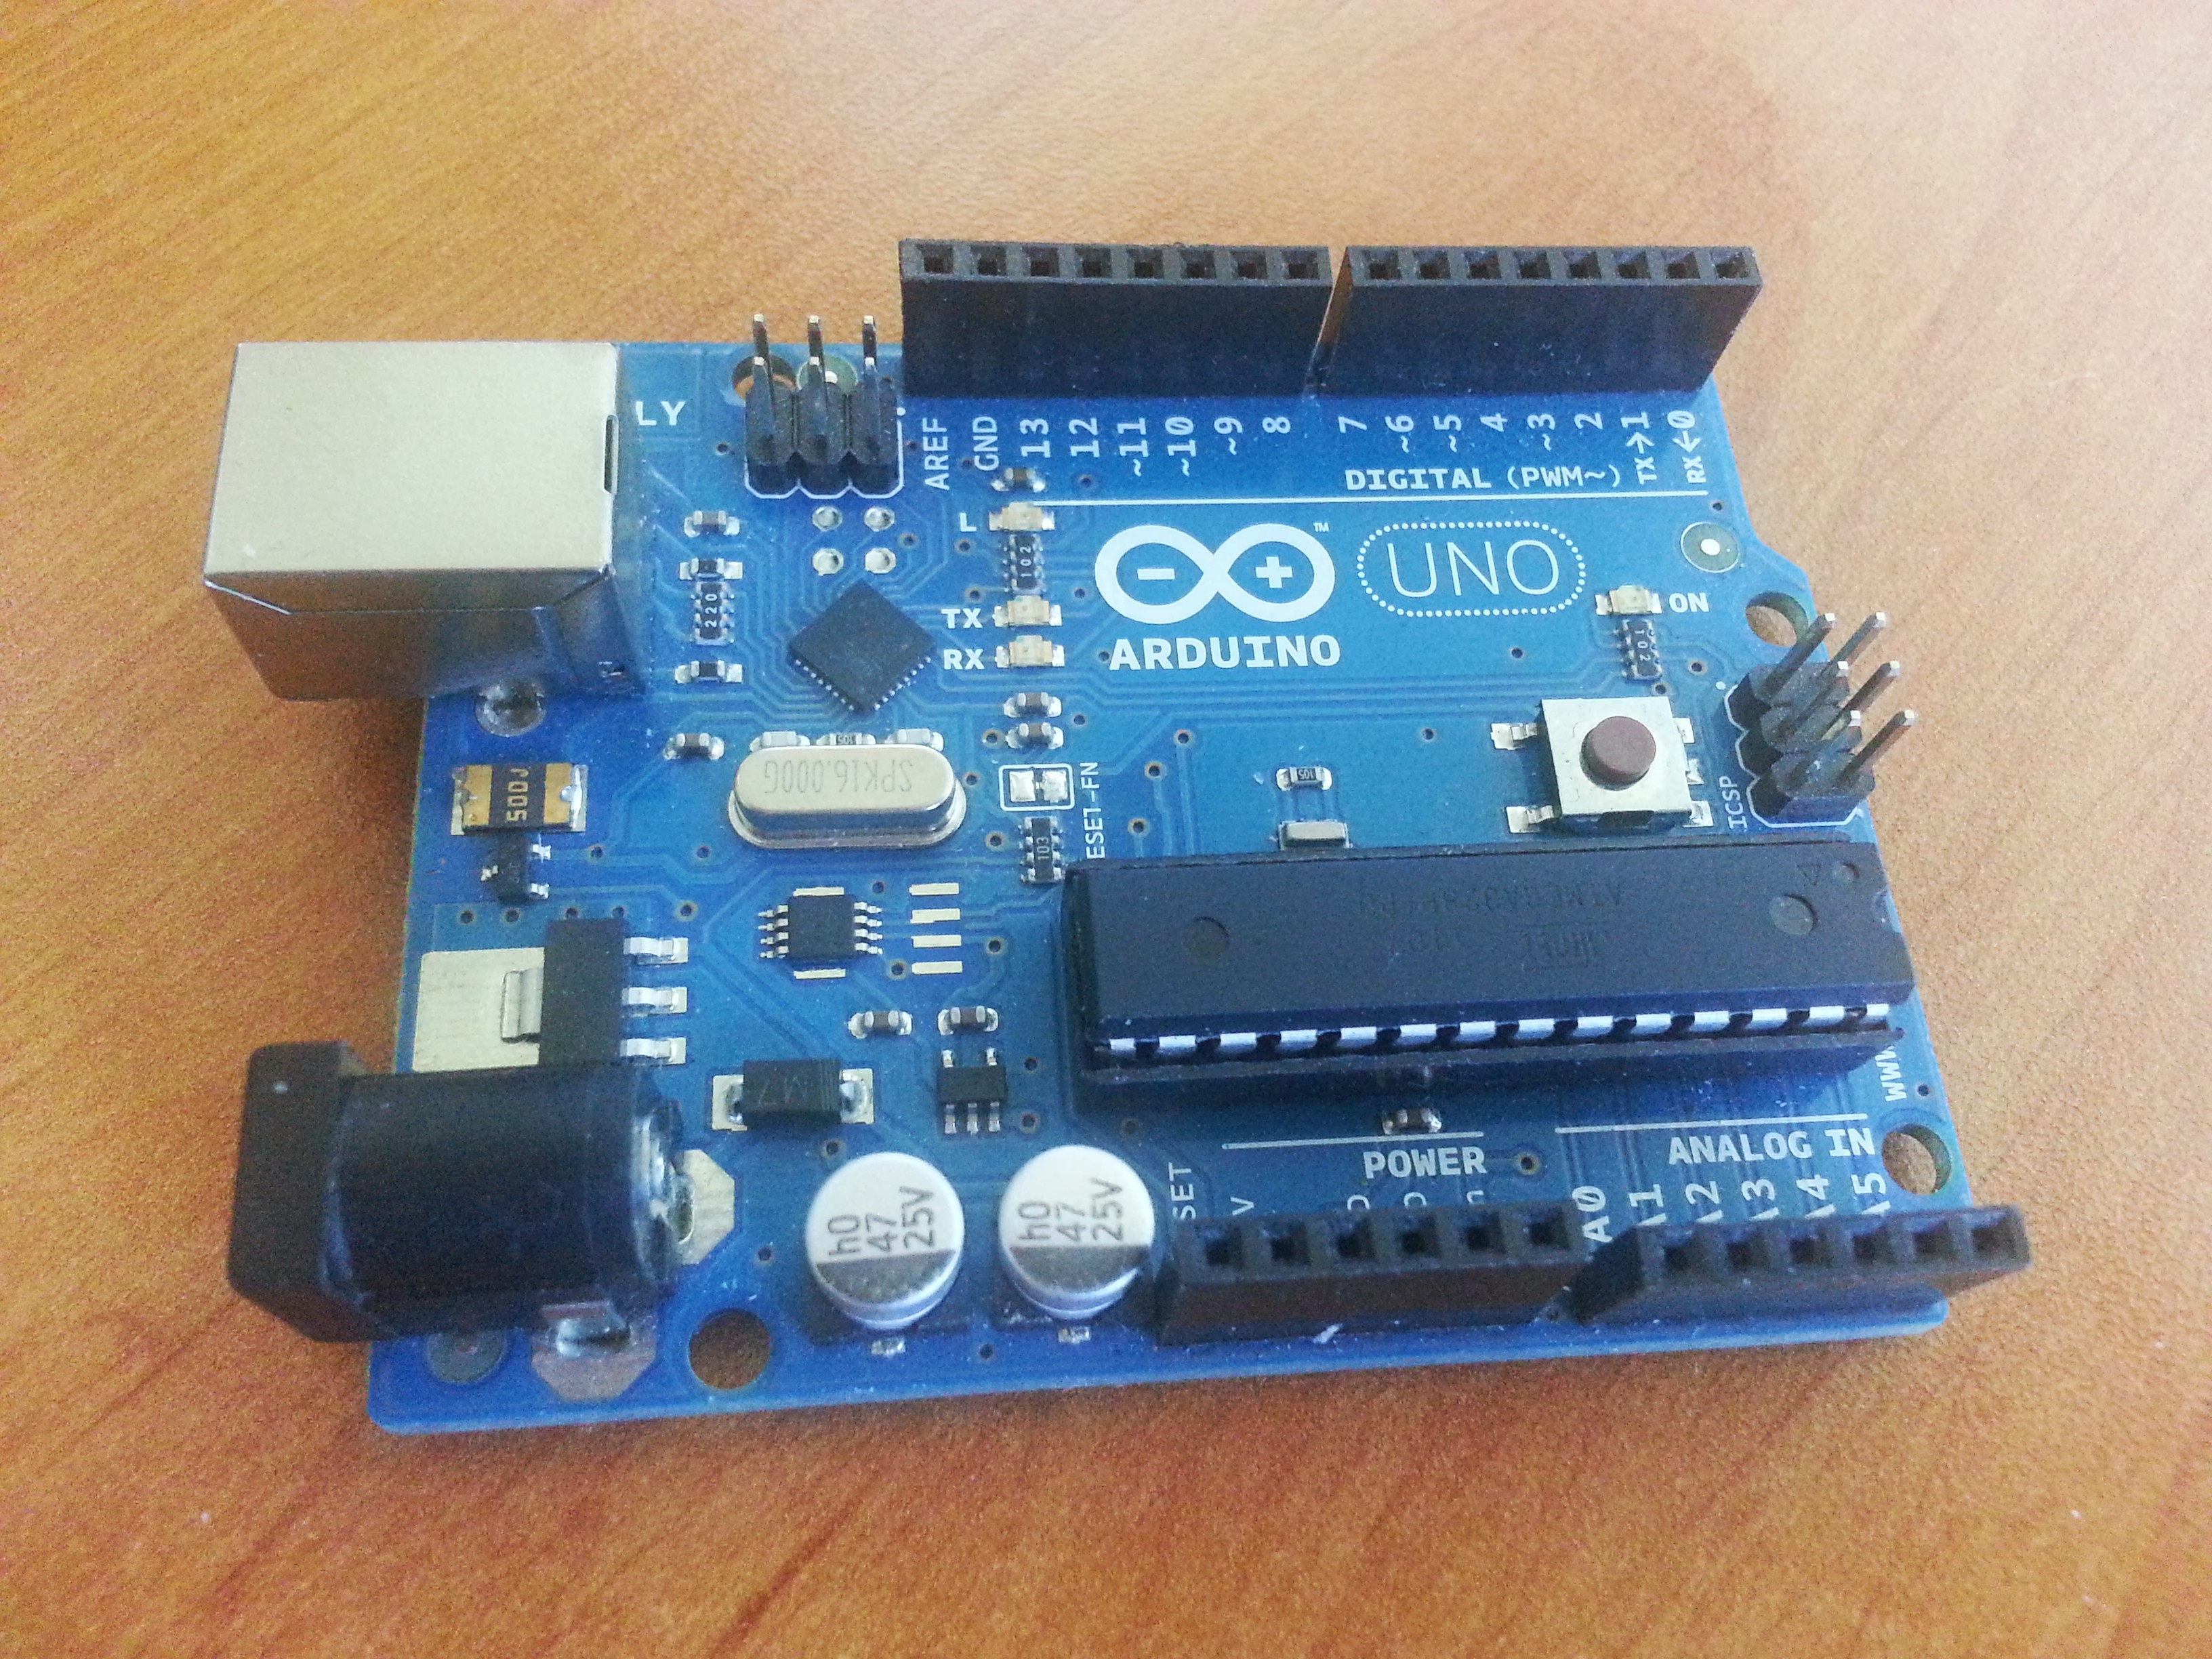
\includegraphics[width=\linewidth/2]{img/arduino.jpg}
    \caption{Un des Arduino utilisé pendant mon stage.}
\end{figure}

~

Ses schématiques sont fournies en PDF et au format EAGLE, et elle est livrée avec un IDE en JAVA permettant de facilement programmer dans le langage «PDE», qui est en fait une simplification et un ensemble de bibliothèques C ou C++ (il est donc également possible de la programmer directement en C ou C++).

\begin{figure}[h!]
    \centering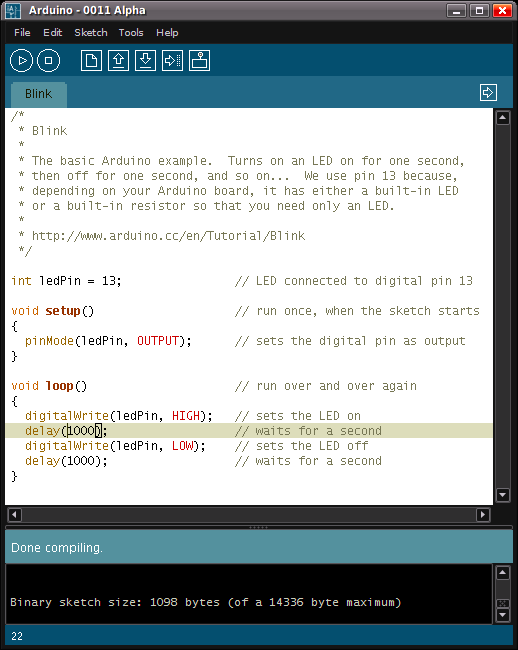
\includegraphics[width=\linewidth/2]{img/arduino_ide.png}
    \caption{Capture d’écran de l’IDE avec le programme «Blink», un exemple permettant de faire clignotter une LED.}
\end{figure}

~

On peut aussi trouver sur certaines cartes des boutons poussoirs et des LEDs intégrés, afin de permettre à un débutant en électronique de comprendre sans avoir à acheter et connecter des composants externes.

~

Sa forme et l’emplacement des ses ports sont conçus de manière à pouvoir facilement ajouter des «Shields» en les empilant sur la carte, ce qui permet d’ajouter à bas coûts des fonctionnalités à la carte de base, comme des séries de convertisseurs, des ports USB ou Ethernet, ou encore des modules WiFi ou GSM.

\begin{figure}[h!]
    \centering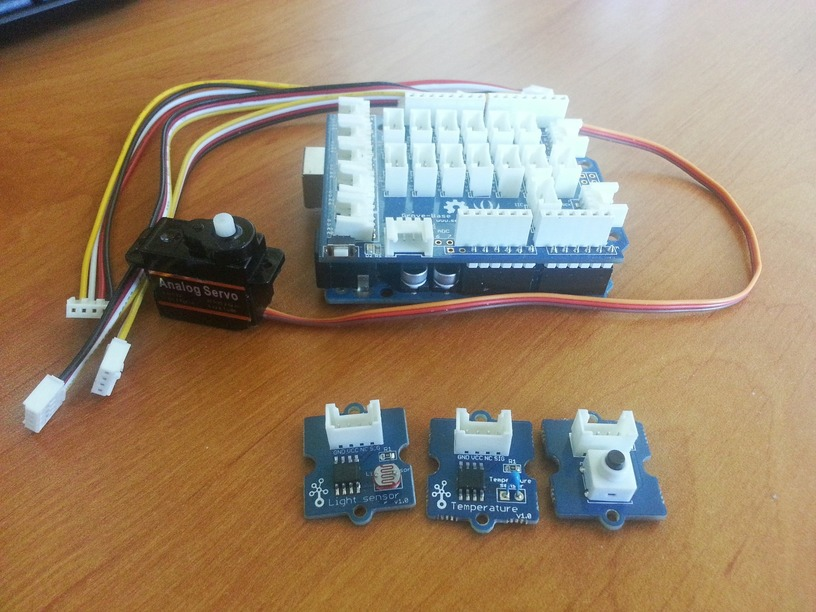
\includegraphics[width=\linewidth/2]{img/arduino_shield.jpg}
    \caption{Un Arduino, un shield constitué simplement de connecteurs et des cateurs et actionneurs.}
\end{figure}


\begin{figure}[h!]
    \centering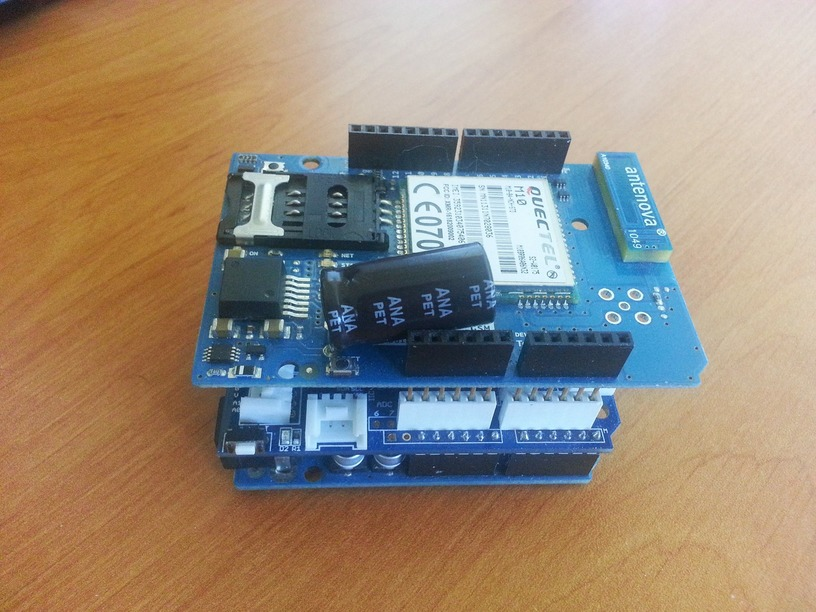
\includegraphics[width=\linewidth/2]{img/gsm.jpg}
    \caption{Un arduino, le shield pour les connecteurs, et un shield GSM empillés.}
\end{figure}


Un grand nombre de cartes différentes, proposant diverses puissances, tailles, consommations et fonctionnalités, de shields et de kits sont disponible sur le \hyperref[http://arduino.cc/en/Main/Products]{site officiel}.

\begin{figure}[h!]
    \centering
\includegraphics{img/logo.png}
    \caption{Arduino: http://arduino.cc}
\end{figure}

\clearpage

\subsection{Shield GSM pour Arduino}
\label{gsm}

L’objectif initial du stage était de faire fonctionner logiciellement un shield GSM pour Raspberry Pi, basé sur un modem 3G Sierra Wireless. Cependant, au moment où j’ai commencé le stage, la carte n’était pas encore conçue, et j’ai proposé de me baser sur le shield GSM pour arduino afin de concevoir une carte équivalente, de manière open-hardware.

\begin{figure}[h!]
    \centering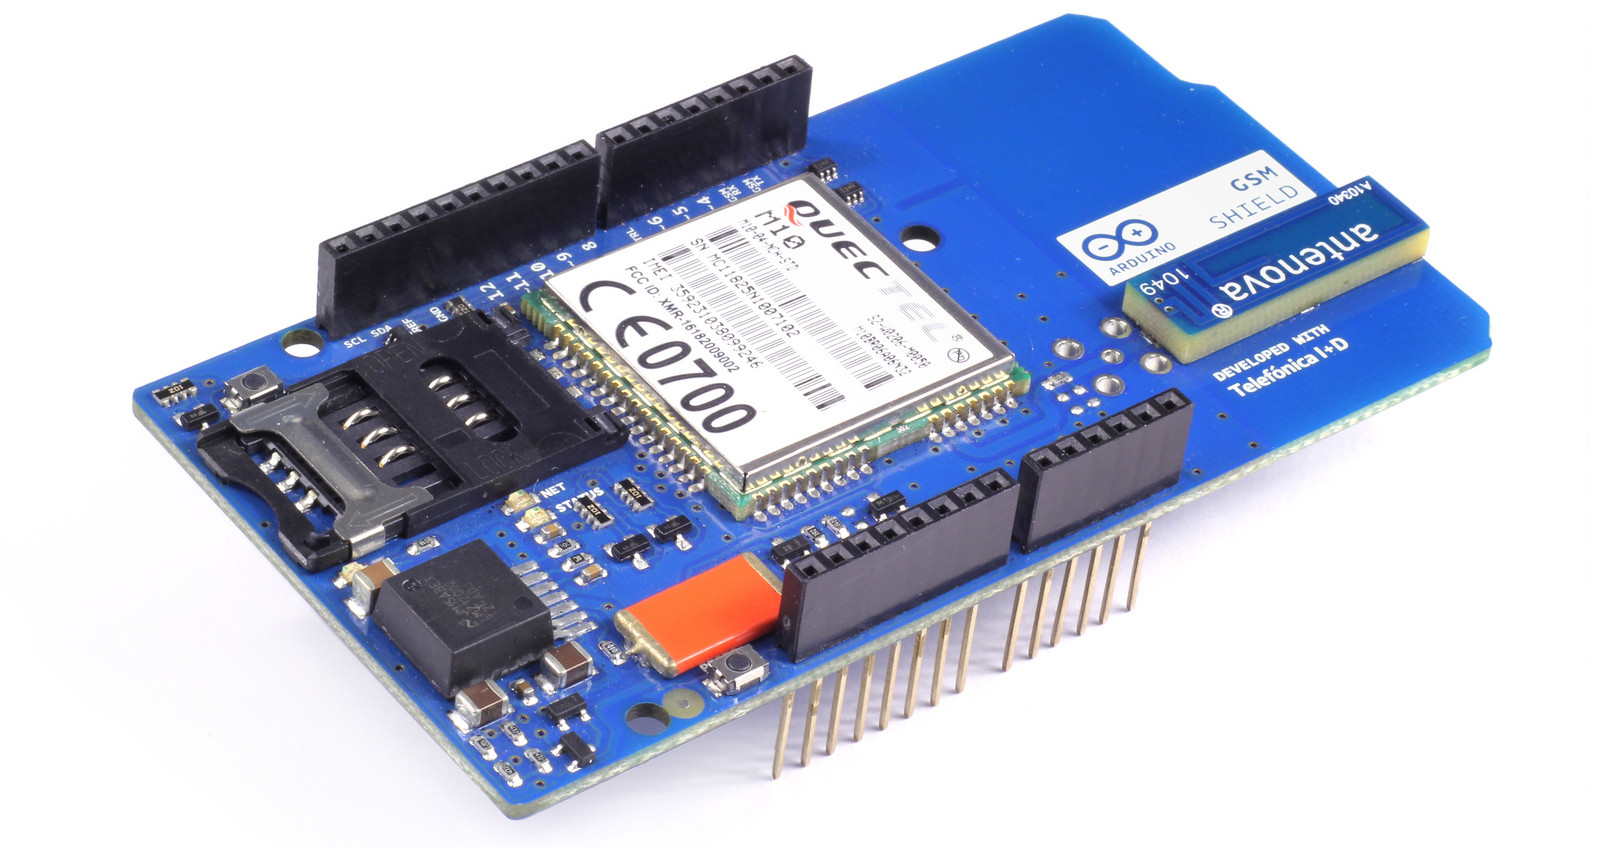
\includegraphics[width=\linewidth*2/3]{img/shield_gsm.jpg}
    \centering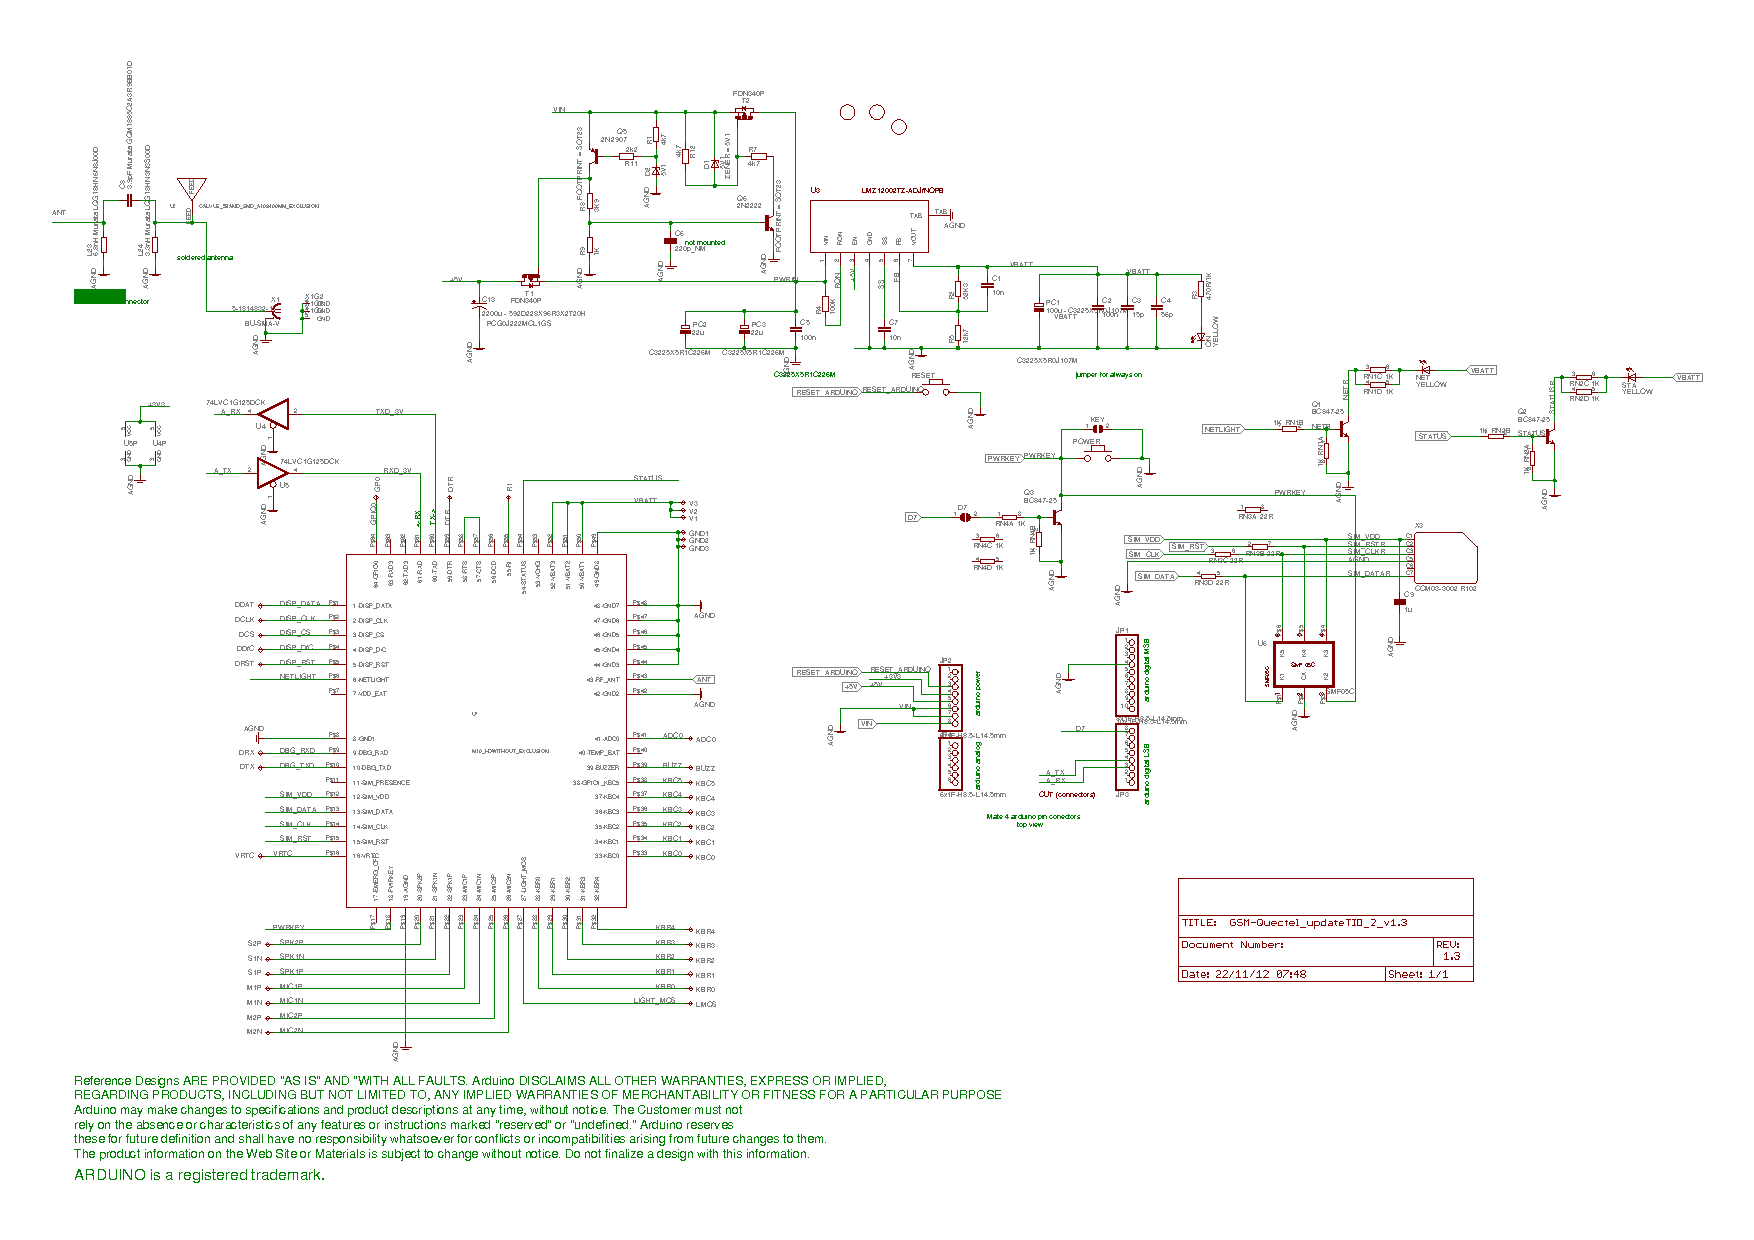
\includegraphics[width=\linewidth]{img/arduino-gsm-shield-schematic.pdf}
    \caption{Le shield GSM pour Arduino, et sa schématique open-hardware.}
\end{figure}

Seuls quelques calculs RF pour l’antenne auraient pu poser problème dans le principe d’open-Hardware, vu que nous avons appris à l’n7 à utiliser les logiciels propriétaires particulièrement couteux, que je ne pouvais donc pas utiliser dans mon stage.

~

Finalement, la conception de cette carte a été laissée à l’entreprise SnootLab.

\clearpage

\subsection{Beagle Bone / Beagle Bone Black}
\label{bbb}

La BeagleBone est un ordinateur faible consommation et open source de Texas Instruments, qui fait la taille d’une carte de crédit. Elle coute environ 90\$, peut se connecter à des réseaux ethernet et à internet, et peut faire tourner des distributions GNU/Linux telles que Debian, Ubuntu, Android ou Angstrom.

Comme l’arduino, ses ports d’entrées sortie sont disposés verticallement sur les bords longs, mais elle dispose de 2 ports de 46 connecteurs.

Elle embarque un processeur ARM tournant à 720MHz, un port ethernet, un port USB host, un lecteur de carte micro-SD pour y installer un système d’exploitation, et un jeu de 4 LEDs permettant de vérifier qu’elle fonctionne, ou d’apprendre à gérer les GPIO sur un ordinateur de ce type.

\begin{figure}[h!]
    \centering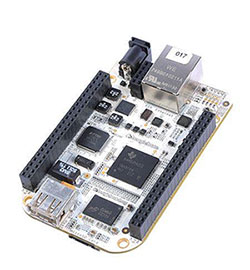
\includegraphics[width=\linewidth/2]{img/bb.jpg}
    \caption{Une BeagleBone, identique à celle utilisée pendant mon stage}
\end{figure}

La BeagleBone Black est une évolution de la BeagleBone dont le PCB est noir plutôt que blanc.

Elle embarque un processeur ARM Cortex-A8 tournant à 1GHz, un port HDMI, une accélération graphique 3D, et ne coûte que 45\$.

\begin{figure}[h!]
    \centering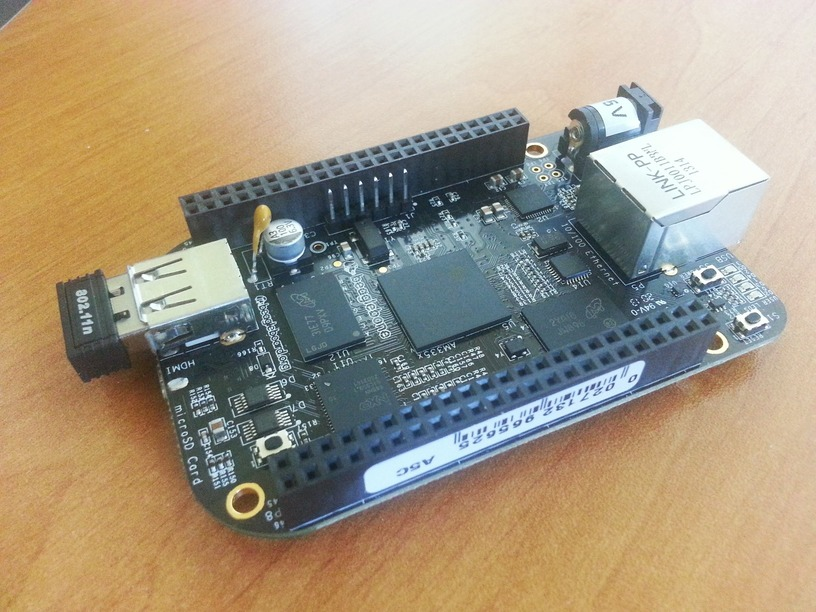
\includegraphics[width=\linewidth/2]{img/bbb.jpg}
    \caption{La BeagleBone Black qui m’a été offerte par les employés de Texas Instruments.}
\end{figure}

\clearpage

\subsection{Eclo}
\label{eclo}

Eclo est un Dev Kit pour le M2M utilisant les technologies open-source de Sierra Wireless.


\begin{figure}[h!]
    \centering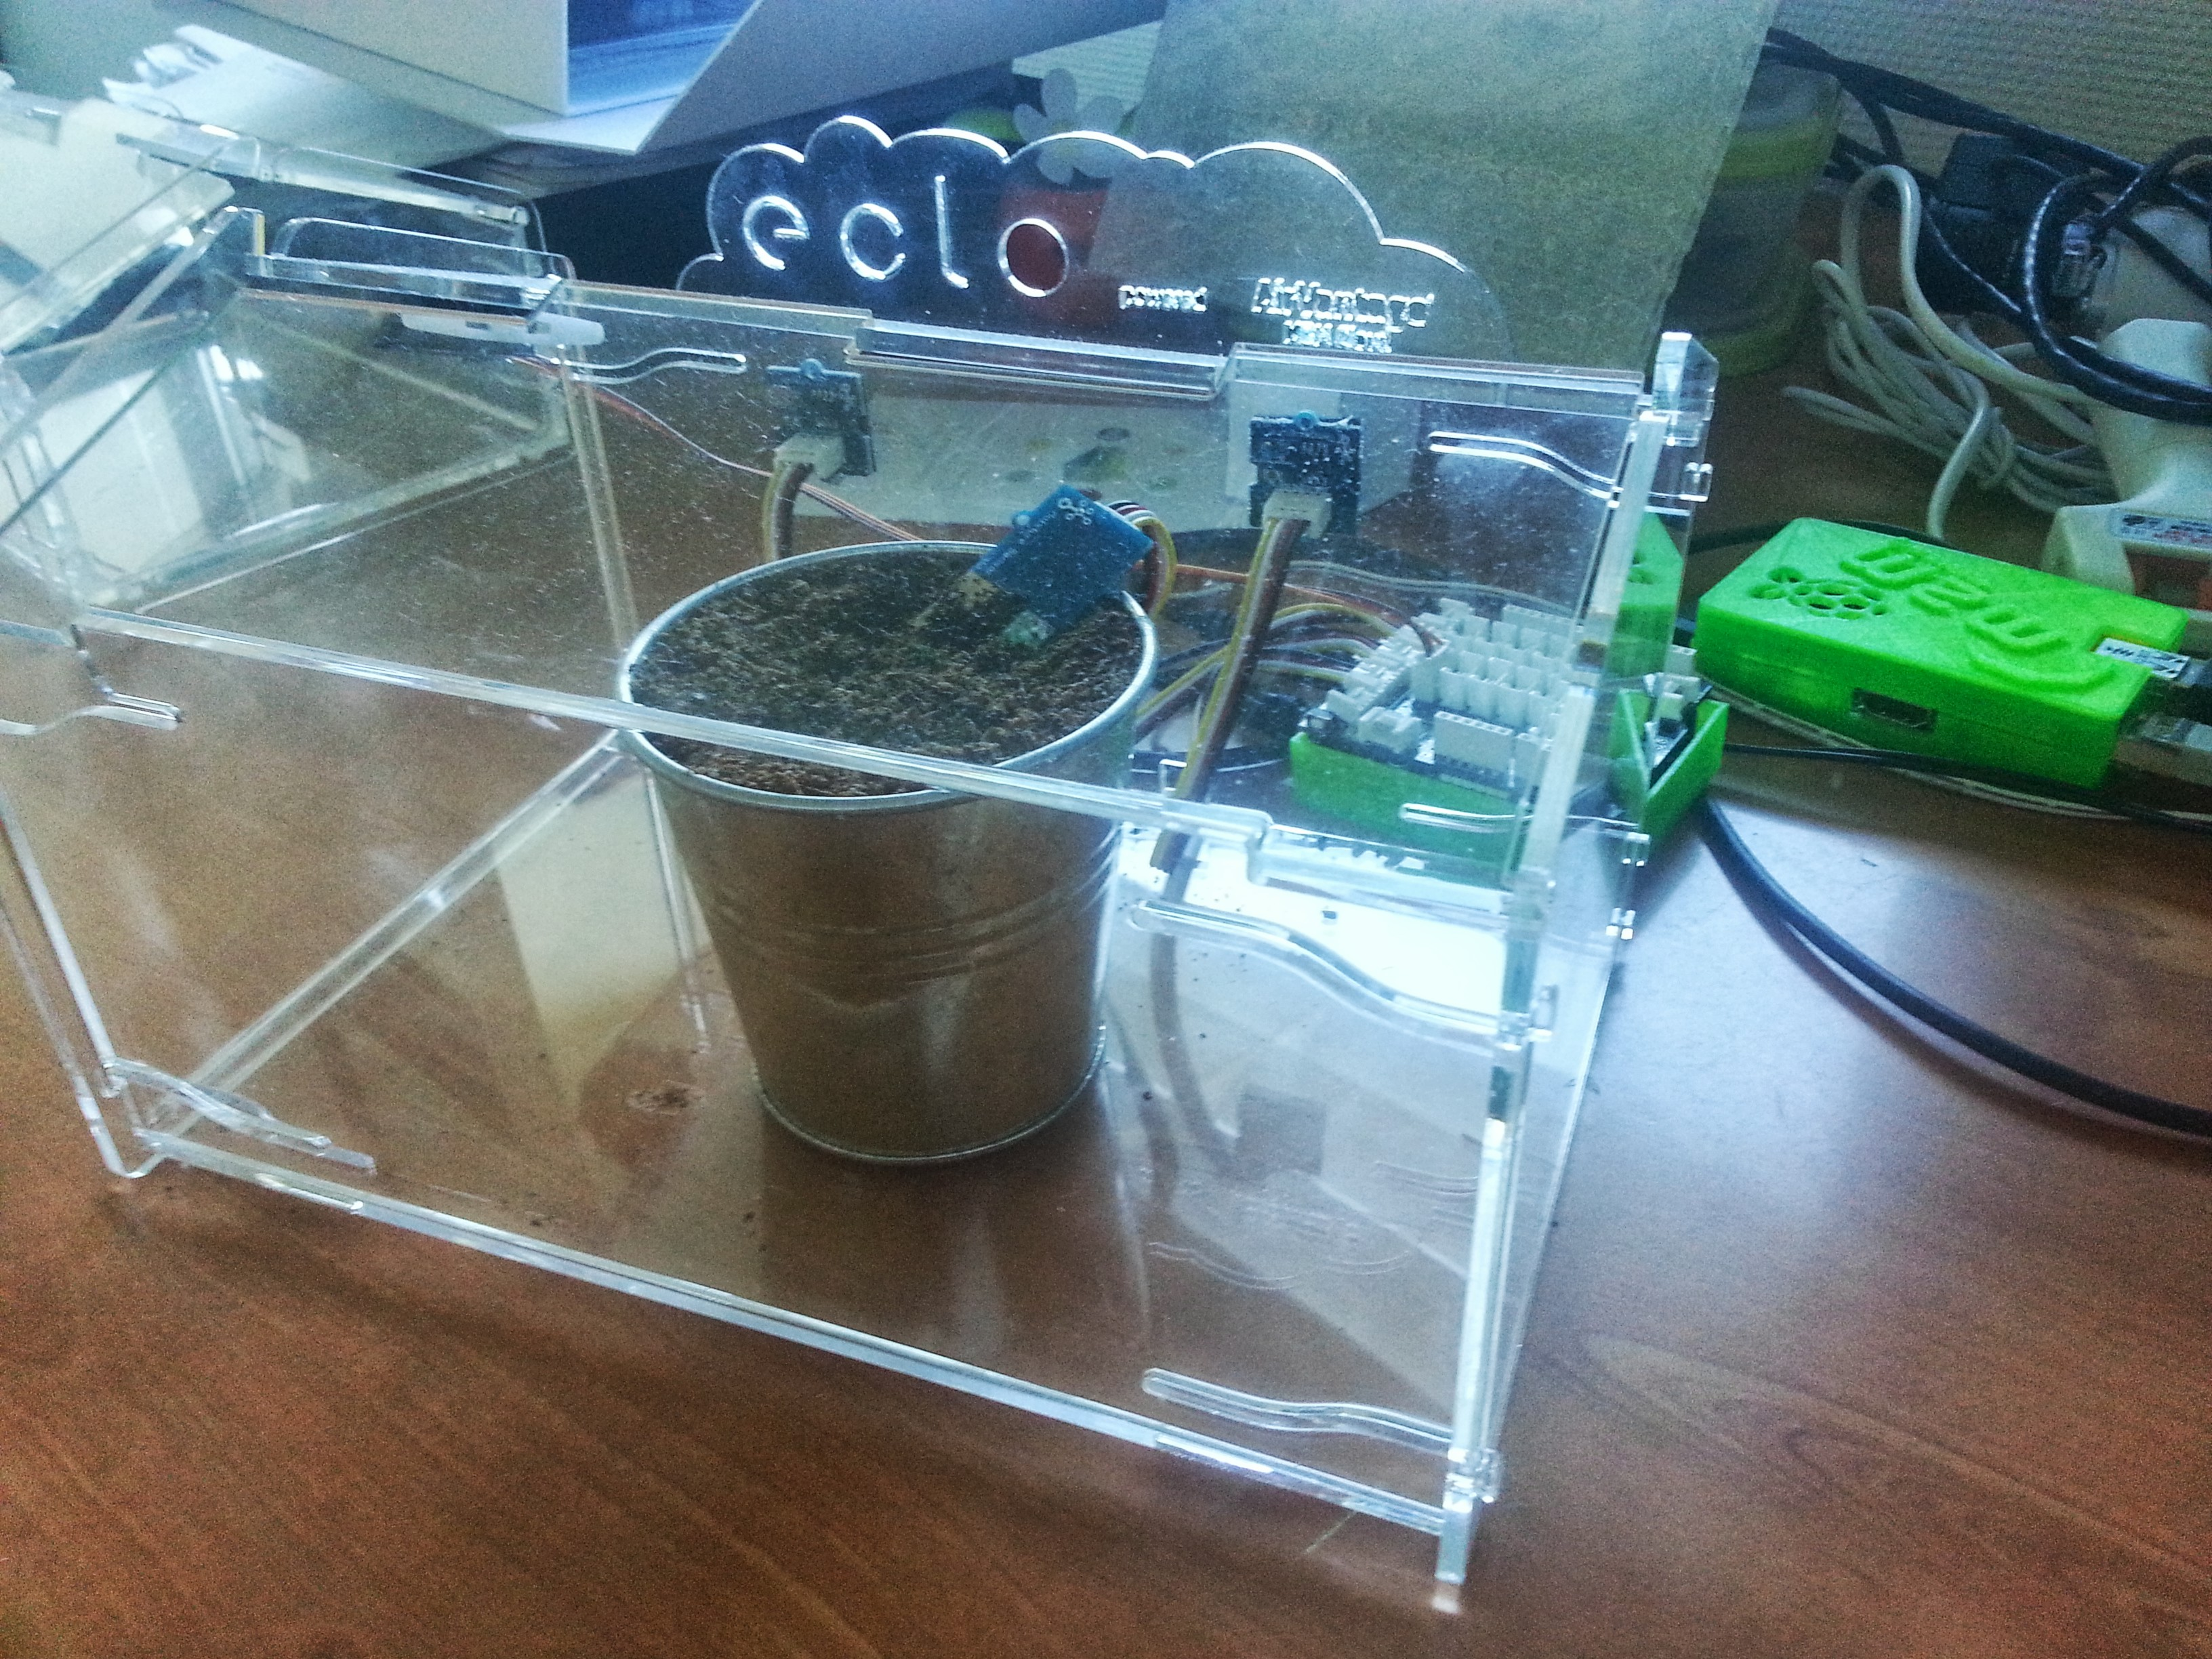
\includegraphics[width=\linewidth*2/3]{img/eclo.jpg}
    \caption{La première version fonctionnelle d’Eclo, dans l’open-space de Labège de Sierra Wireless}
\end{figure}

Prévu pour être vendu à prix coutant (aux alentours de 100€), ce Dev Kit se compose d’une serre design en plexiglass découpé au laser, d’un Raspberry Pi, et d’un Arduino pour la partie embarquée, assisté d’un shield de connecteurs.

\begin{figure}[h!]
    \centering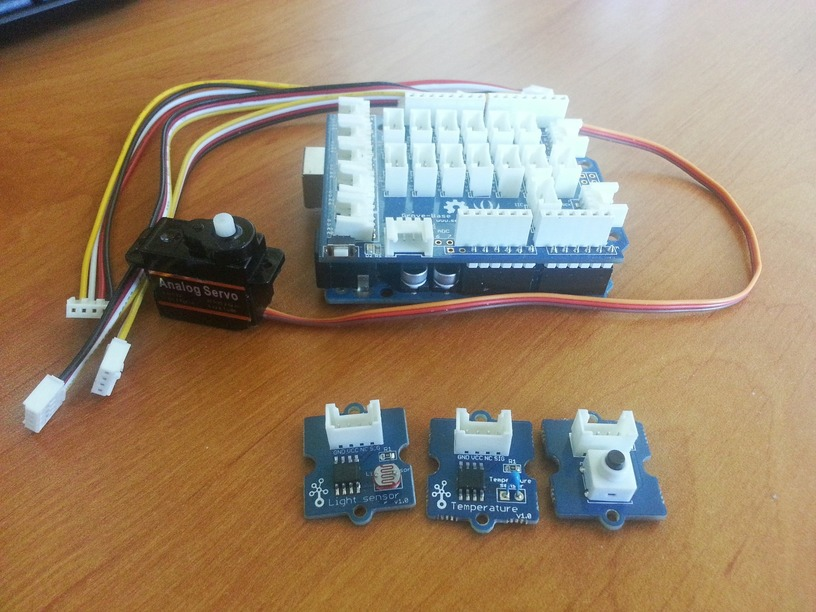
\includegraphics[width=\linewidth*2/3]{img/arduino_shield.jpg}
    \caption{L’arduino, le shield, les capteurs et actionneurs et la connectique fournis avec eclo}
\end{figure}

\clearpage

\subsection{mbed}
\label{mbed}

mbed est une plateforme de développement. Ceci comprend un écosystème d’application web, avec son IDE en ligne, son gestionnaire de versions, son réseau social et sa collection d’applications et de librairies ; mais aussi un regroupement industriel autour des microcontrolleurs ARM, comprenant entre autres NXP, Freescale et bien sûr ARM.

Ce regroupement industriel propose un ensemble étéroclyte de cartes de développement, mais l’on désigne par abus de langage la carte «mbed LPC1768» par «mbed».

\begin{figure}[h!]
    \centering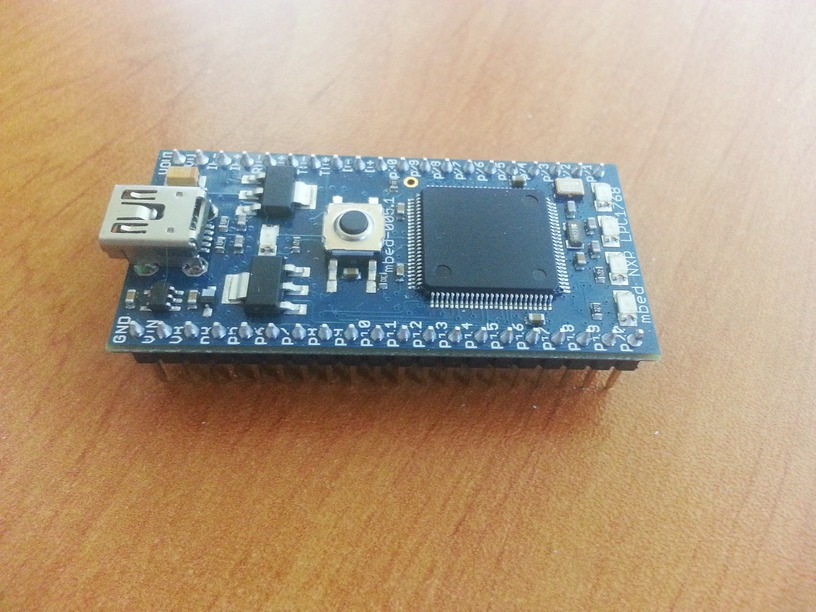
\includegraphics[width=\linewidth*2/3]{img/mbed.jpg}
    \caption{La carte mbed utilisée pendant mon stage.}
\end{figure}

Cette carte mbed open-hardware embarque un ARM Cortex-M3 cadencé à 96MHz, un circuit d’alimentation (USB ou 9V), un système de programmation simplifié en USB (la carte apparait comme un péréphérique de stockage, et on n’a qu’à y déposer le fichier binaire compilé par l’IDE en ligne), et un grand nombre de fonctionnalités connectées sur les entrées/sorties et les 4 LEDs incluses:

\begin{figure}[h!]
    \centering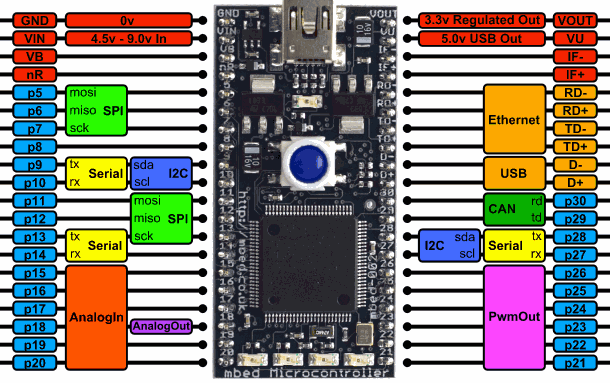
\includegraphics[width=\linewidth*3/4]{img/pinout.png}
    \caption{La connectique de cette carte mbed.}
\end{figure}

\clearpage

\subsection{Extension pour mbed}
\label{mbed_ext}

Contrairement aux Arduino, aux BeagleBone et au RaspberryPi, les ports d’extension de la carte mbed ne sont pas des femelles dans lesquelles on vient brancher des fils comme sur une plaquette labdec ou des shields, mais des males. On peut donc enficher cette carte directement dans un ensemble plus complet, ou bien dans une carte d’extension.

~

C’est le cas de la carte d’extension dont nous disposions:

\begin{figure}[h!]
    \centering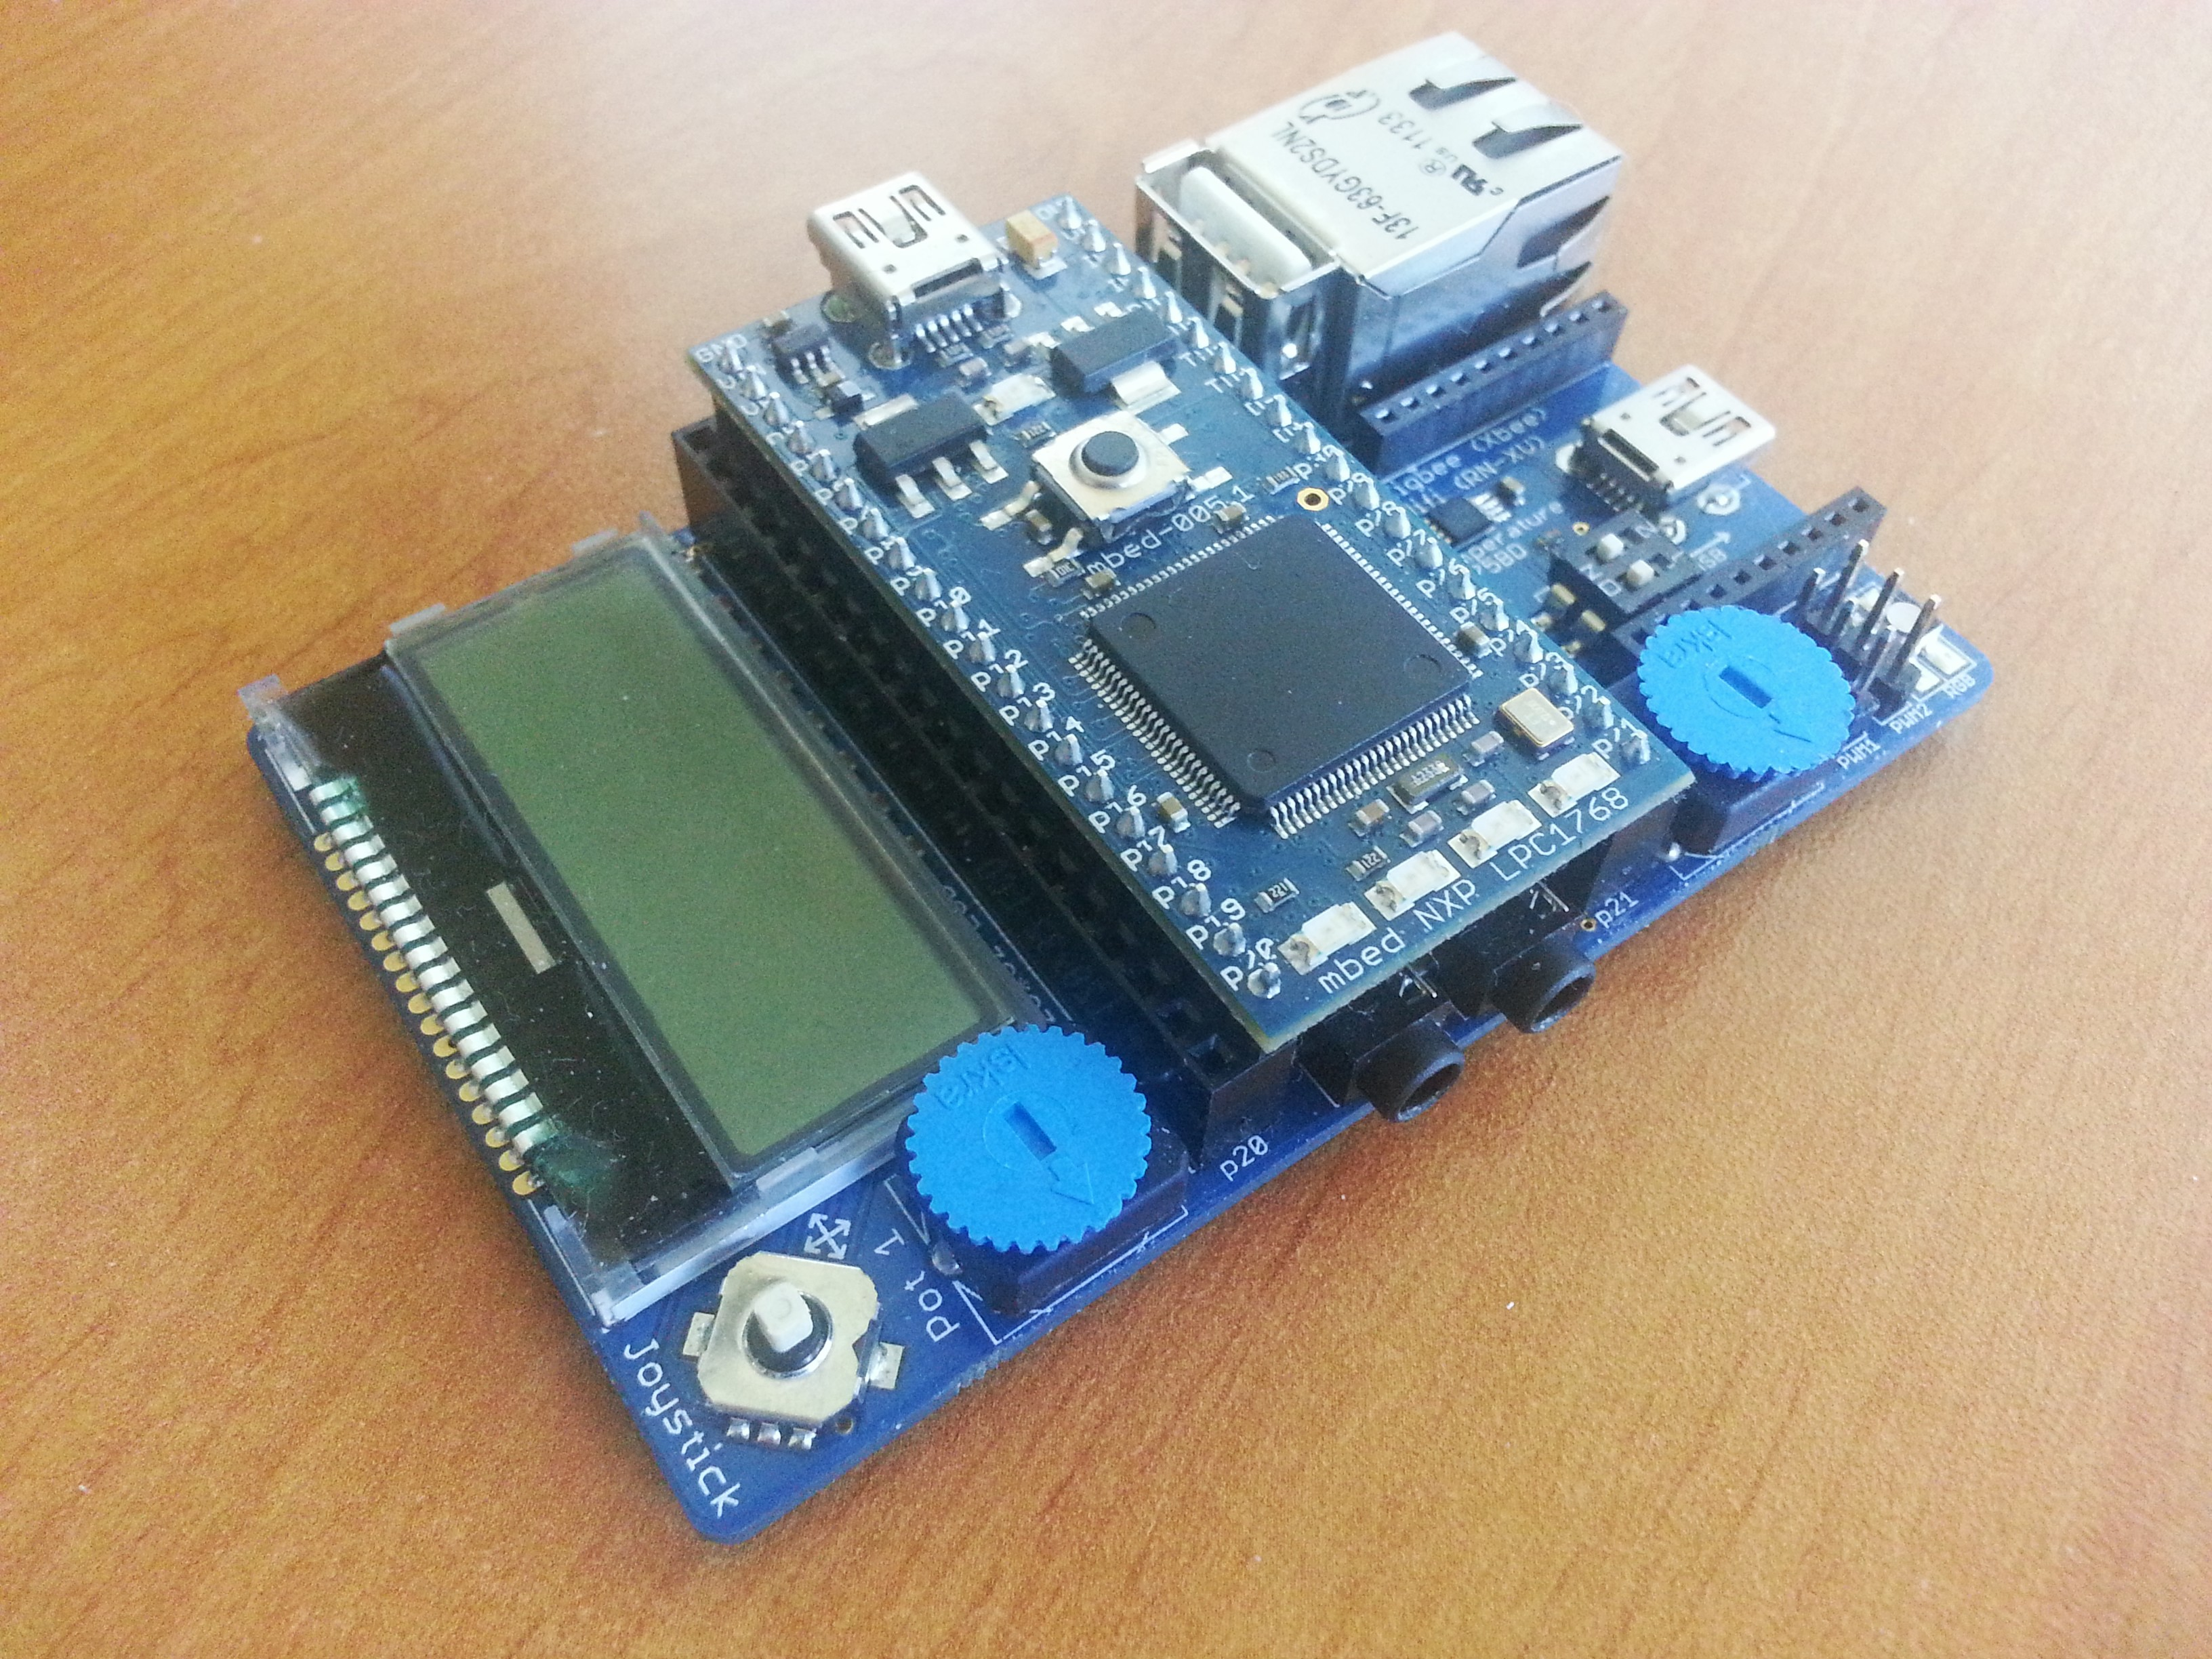
\includegraphics[width=\linewidth*2/3]{img/mbed_ext.jpg}
    \caption{La carte d’extiension pour mbed, avec la carte mbed conectée.}
\end{figure}

~

Cette carte d’extension propose un écran LCD, un joystick, un accéléromètre, un gyroscope, un thermomètre, deux potentiomètres, une LED RGB, deux jack connectés sur un convertisseur analogique/numérique et un convertisseur numérique/analogique (pour faire une sortie casque et une entrée micro), un socket XBEE, un port Ethernet et deux ports USB pouvant être configurés en hôte ou en périphérique.

\begin{figure}[h!]
    \centering
\includegraphics{img/mbed_logo.png}
    \caption{mbed: http://mbed.org}
\end{figure}

\clearpage

\subsection{Freescale KL25Z}
\label{freescale}

Nous disposons également de trois cartes de développement Freescale KL25Z (dite «Freescale Freedom Development Platform») au club robotique de l’école, que j’ai donc pu utiliser lors de mon stage. Elles comprennent entre autres particularités intéressantes une LED RGB particulièrement lumineuse, un «slider» tactile, un accéléromètre, et un microcontroleur cadencé à 48 MHz.

~

Ces cartes ne coûtent que 13\$ pièces, mais les trois que nous avons nous ont été offertes lors de la coupe de robotique Freescale.

~

\begin{figure}[h!]
    \centering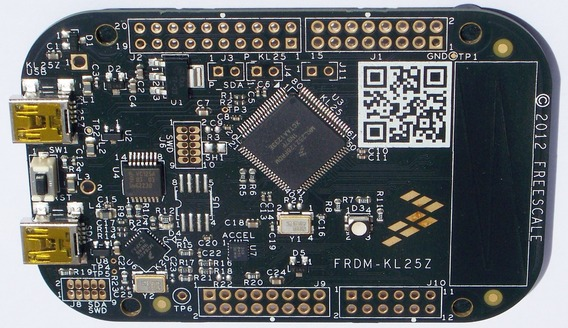
\includegraphics[width=\linewidth*2/3]{img/freescale.jpg}
    \caption{La carte FRDM-KL25Z de Freescale.}
\end{figure}

\begin{figure}[h!]
    \centering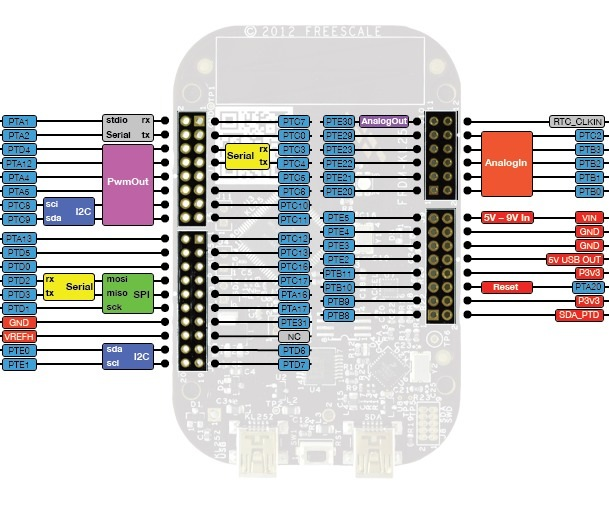
\includegraphics[width=\linewidth*2/3]{img/kl25z-pinout.jpg}
    \caption{Les connecteurs de la carte KL25Z}
\end{figure}

\clearpage

\subsection{Raspberry Pi}
\label{rpi}

La Raspberry Pi est un ordinateur de la taille d’une carte de crédit, conçue par Eben Upton, Rob Mullins, Jack Lang et Alan Mycroft de la faculté d’informatique de l’Université de Cambridge.

L’idée de cette carte est de créer un ordinateur dédié à l’apprentissage de l’informatique aux enfants à très bas prix (deux modèles sont disponible, à 25\$ et 35\$).

~

Elle est open-hardware (bien que basée sur un Broadcom BCM2835, un ARM 11 propriétaire), et dispose de 26 GPIOs, de connecteurs LVDS pour un écran plat et une webcam, d’un port HDMI, d’une sortie vidéo analogique, d’un port Ethernet, de deux ports USB et d’un lecteur de carte SD pour le système d’exploitation.

Cette carte a connu un très gros succès lors de son lancement (et notamment une rupture de stock pendant les quatre mois qui ont suivi), et est désormais fabriquée en angleterre. Divers programmes existent pour en offrir à des écoles ou à des enfants du tiers-monde. Même si elle a d’abord un but éducatif, elle est très appréciée dans les mondes de la domotique, de la robotique, des réseaux et de l’administration système.

~

On peut y utiliser des distributions GNU/Linux telles que Debian (Raspbian), ArchLinux (ArchLinuxARM), Android, Fédora (Pidora), RISC OS, FreeBSD, NetBSD ou encore RaspBMC pour une utilisation en media center.

~

\begin{figure}[h!]
    \centering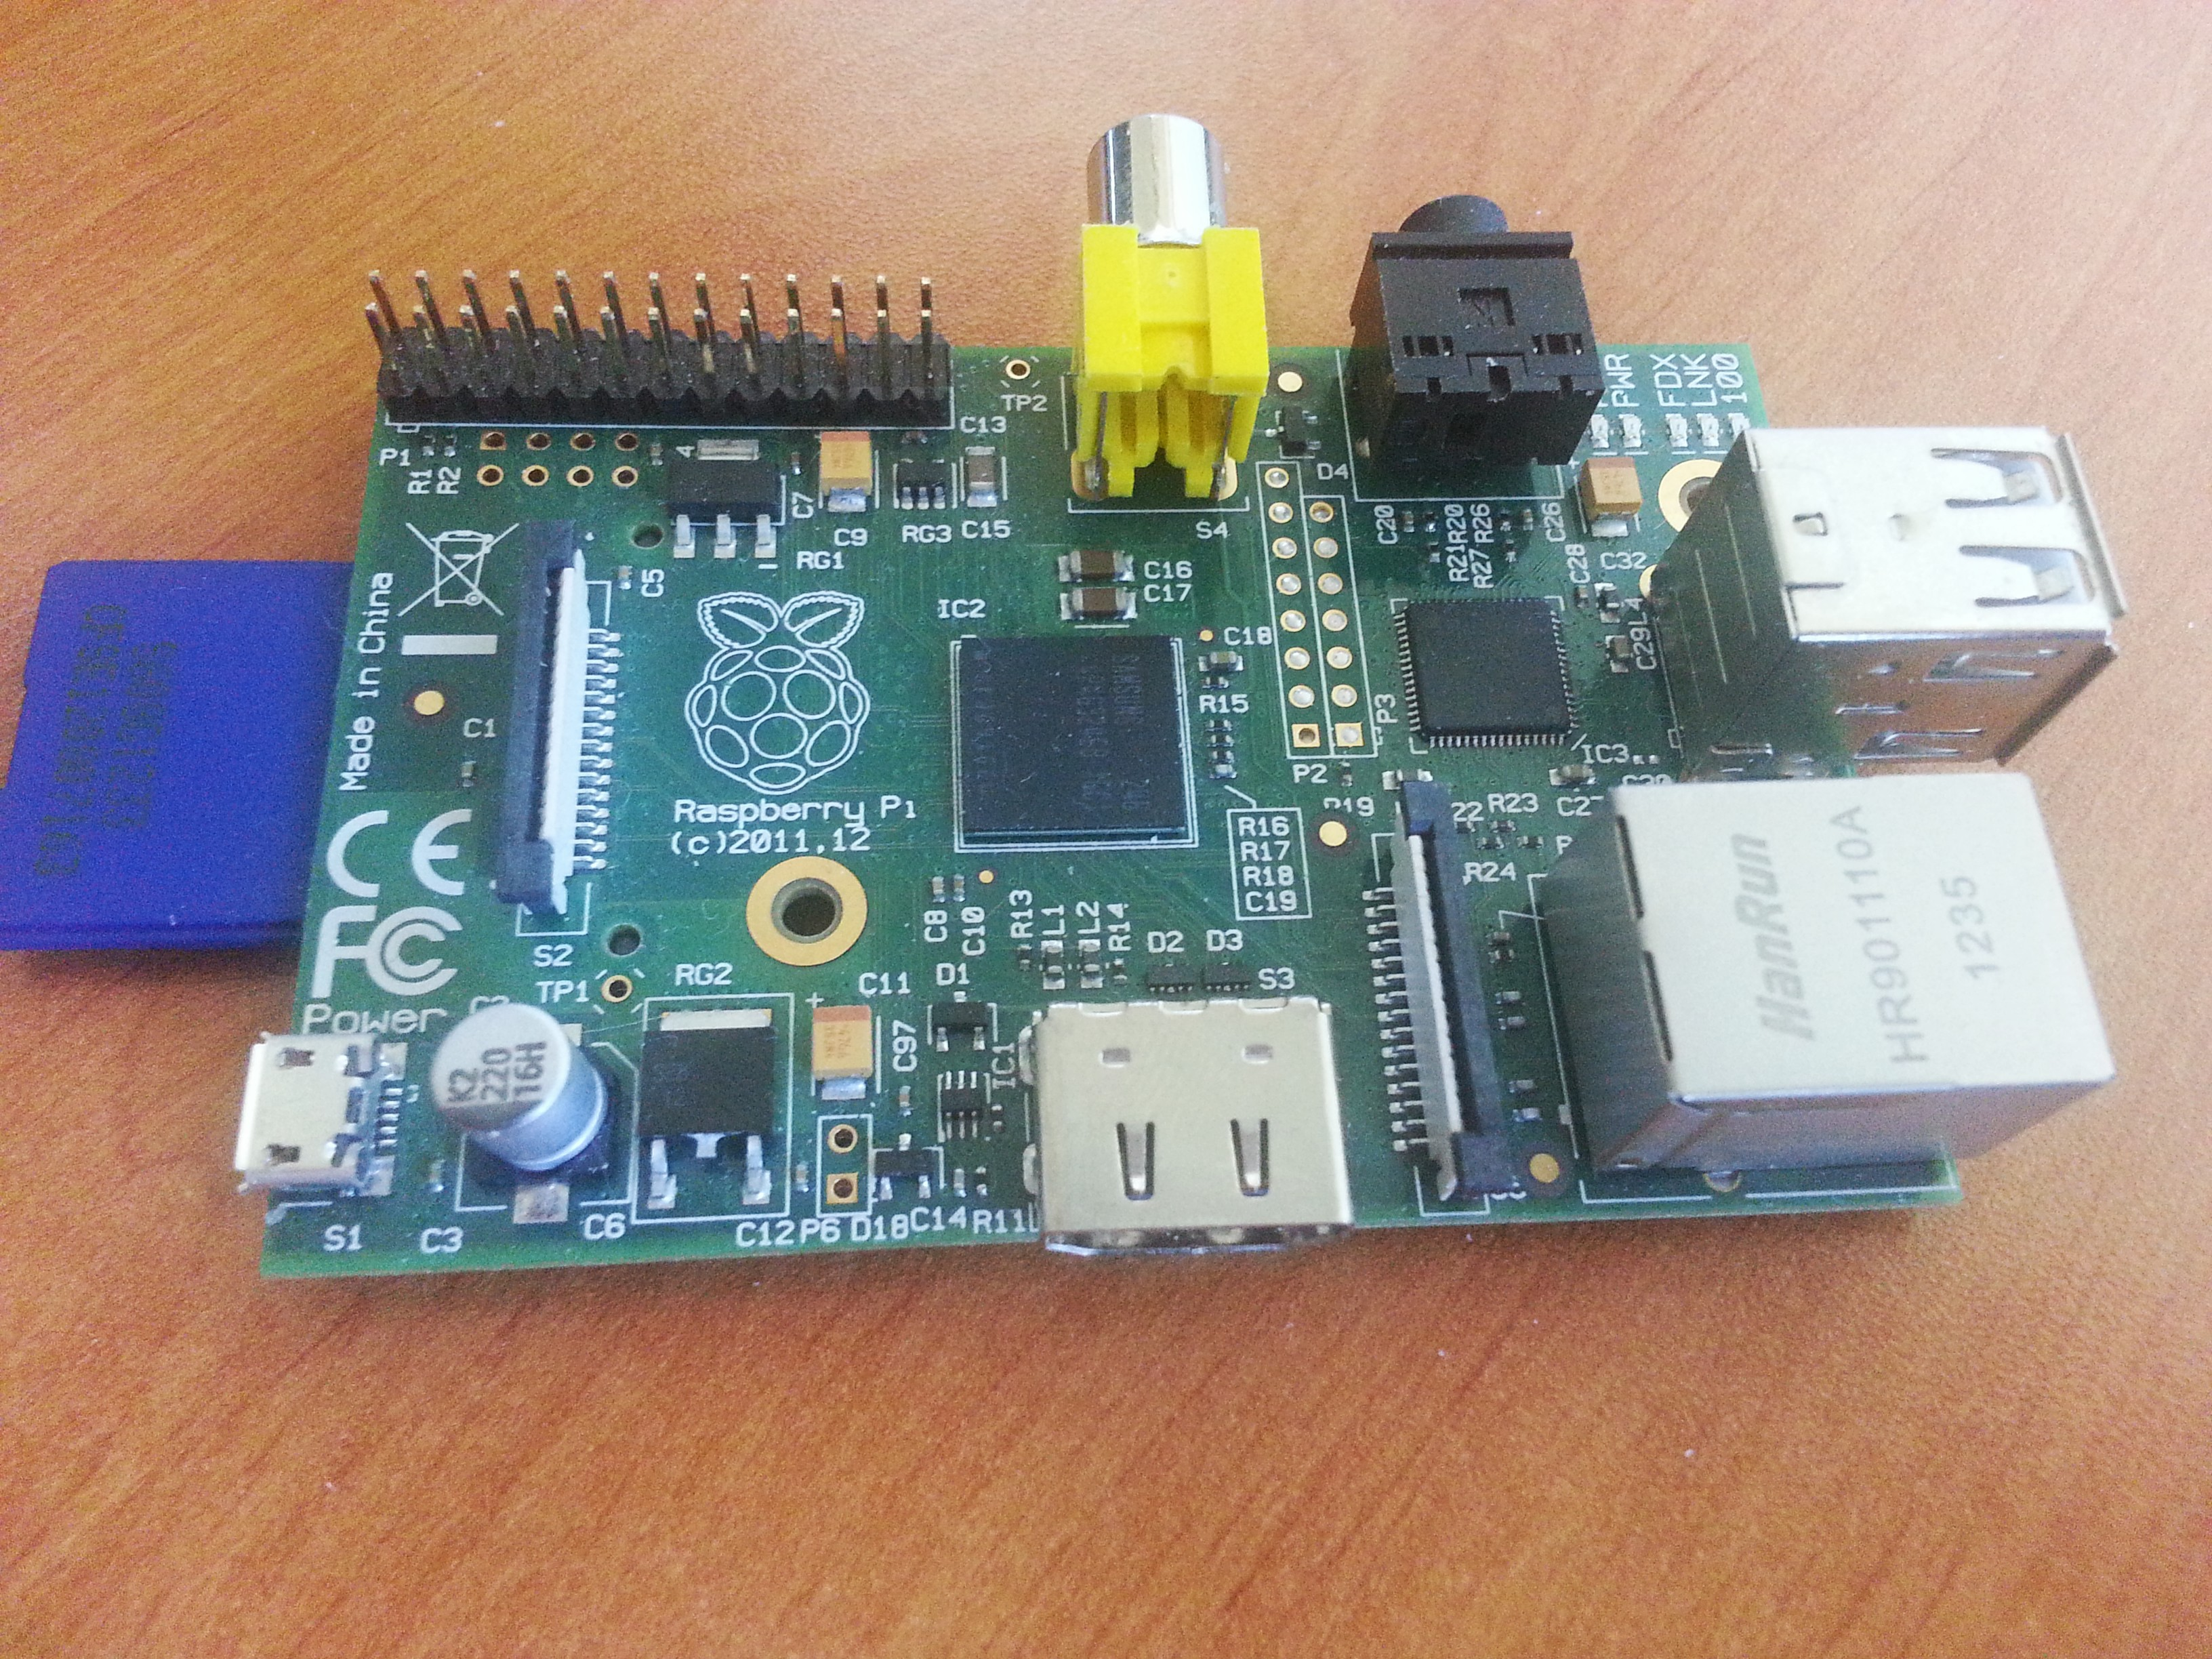
\includegraphics[width=\linewidth*2/3]{img/rpi.jpg}
    \caption{Une des Raspberry Pi (modèle B rev 2) utilisées lors du stage.}
\end{figure}

~

\begin{figure}[h!]
    \centering
\includegraphics[width=\linewidth*2/3]{img/sprite.png}
    \caption{Raspberry Pi: http://www.raspberrypi.org}
\end{figure}

\clearpage

\subsection{XBEE}
\label{xbee}

XBEE est une marque de Digi Internationnal correspondant à une famille de modems ZigBee. Généralement, ces modems ont un facteur de forme commun et sont compatibles pin à pin, ce qui permet facilement de les changer, voire de mettre un modem autre que ZigBee à la place (par exemple WiFi ou GSM).

~

Ces modems implémentent les deux types de topologies proposées par le protocole ZigBee (Mesh et point à point), et ont une portée allant d’une centaine de mètres à 80km.

~

Ils sont particulièrement appréciés en M2M et pour l’IoT, bien que les protocoles qu’ils implémentent ne gèrent généralement pas de sécurités cryptographiques.

~

\begin{figure}[h!]
    \centering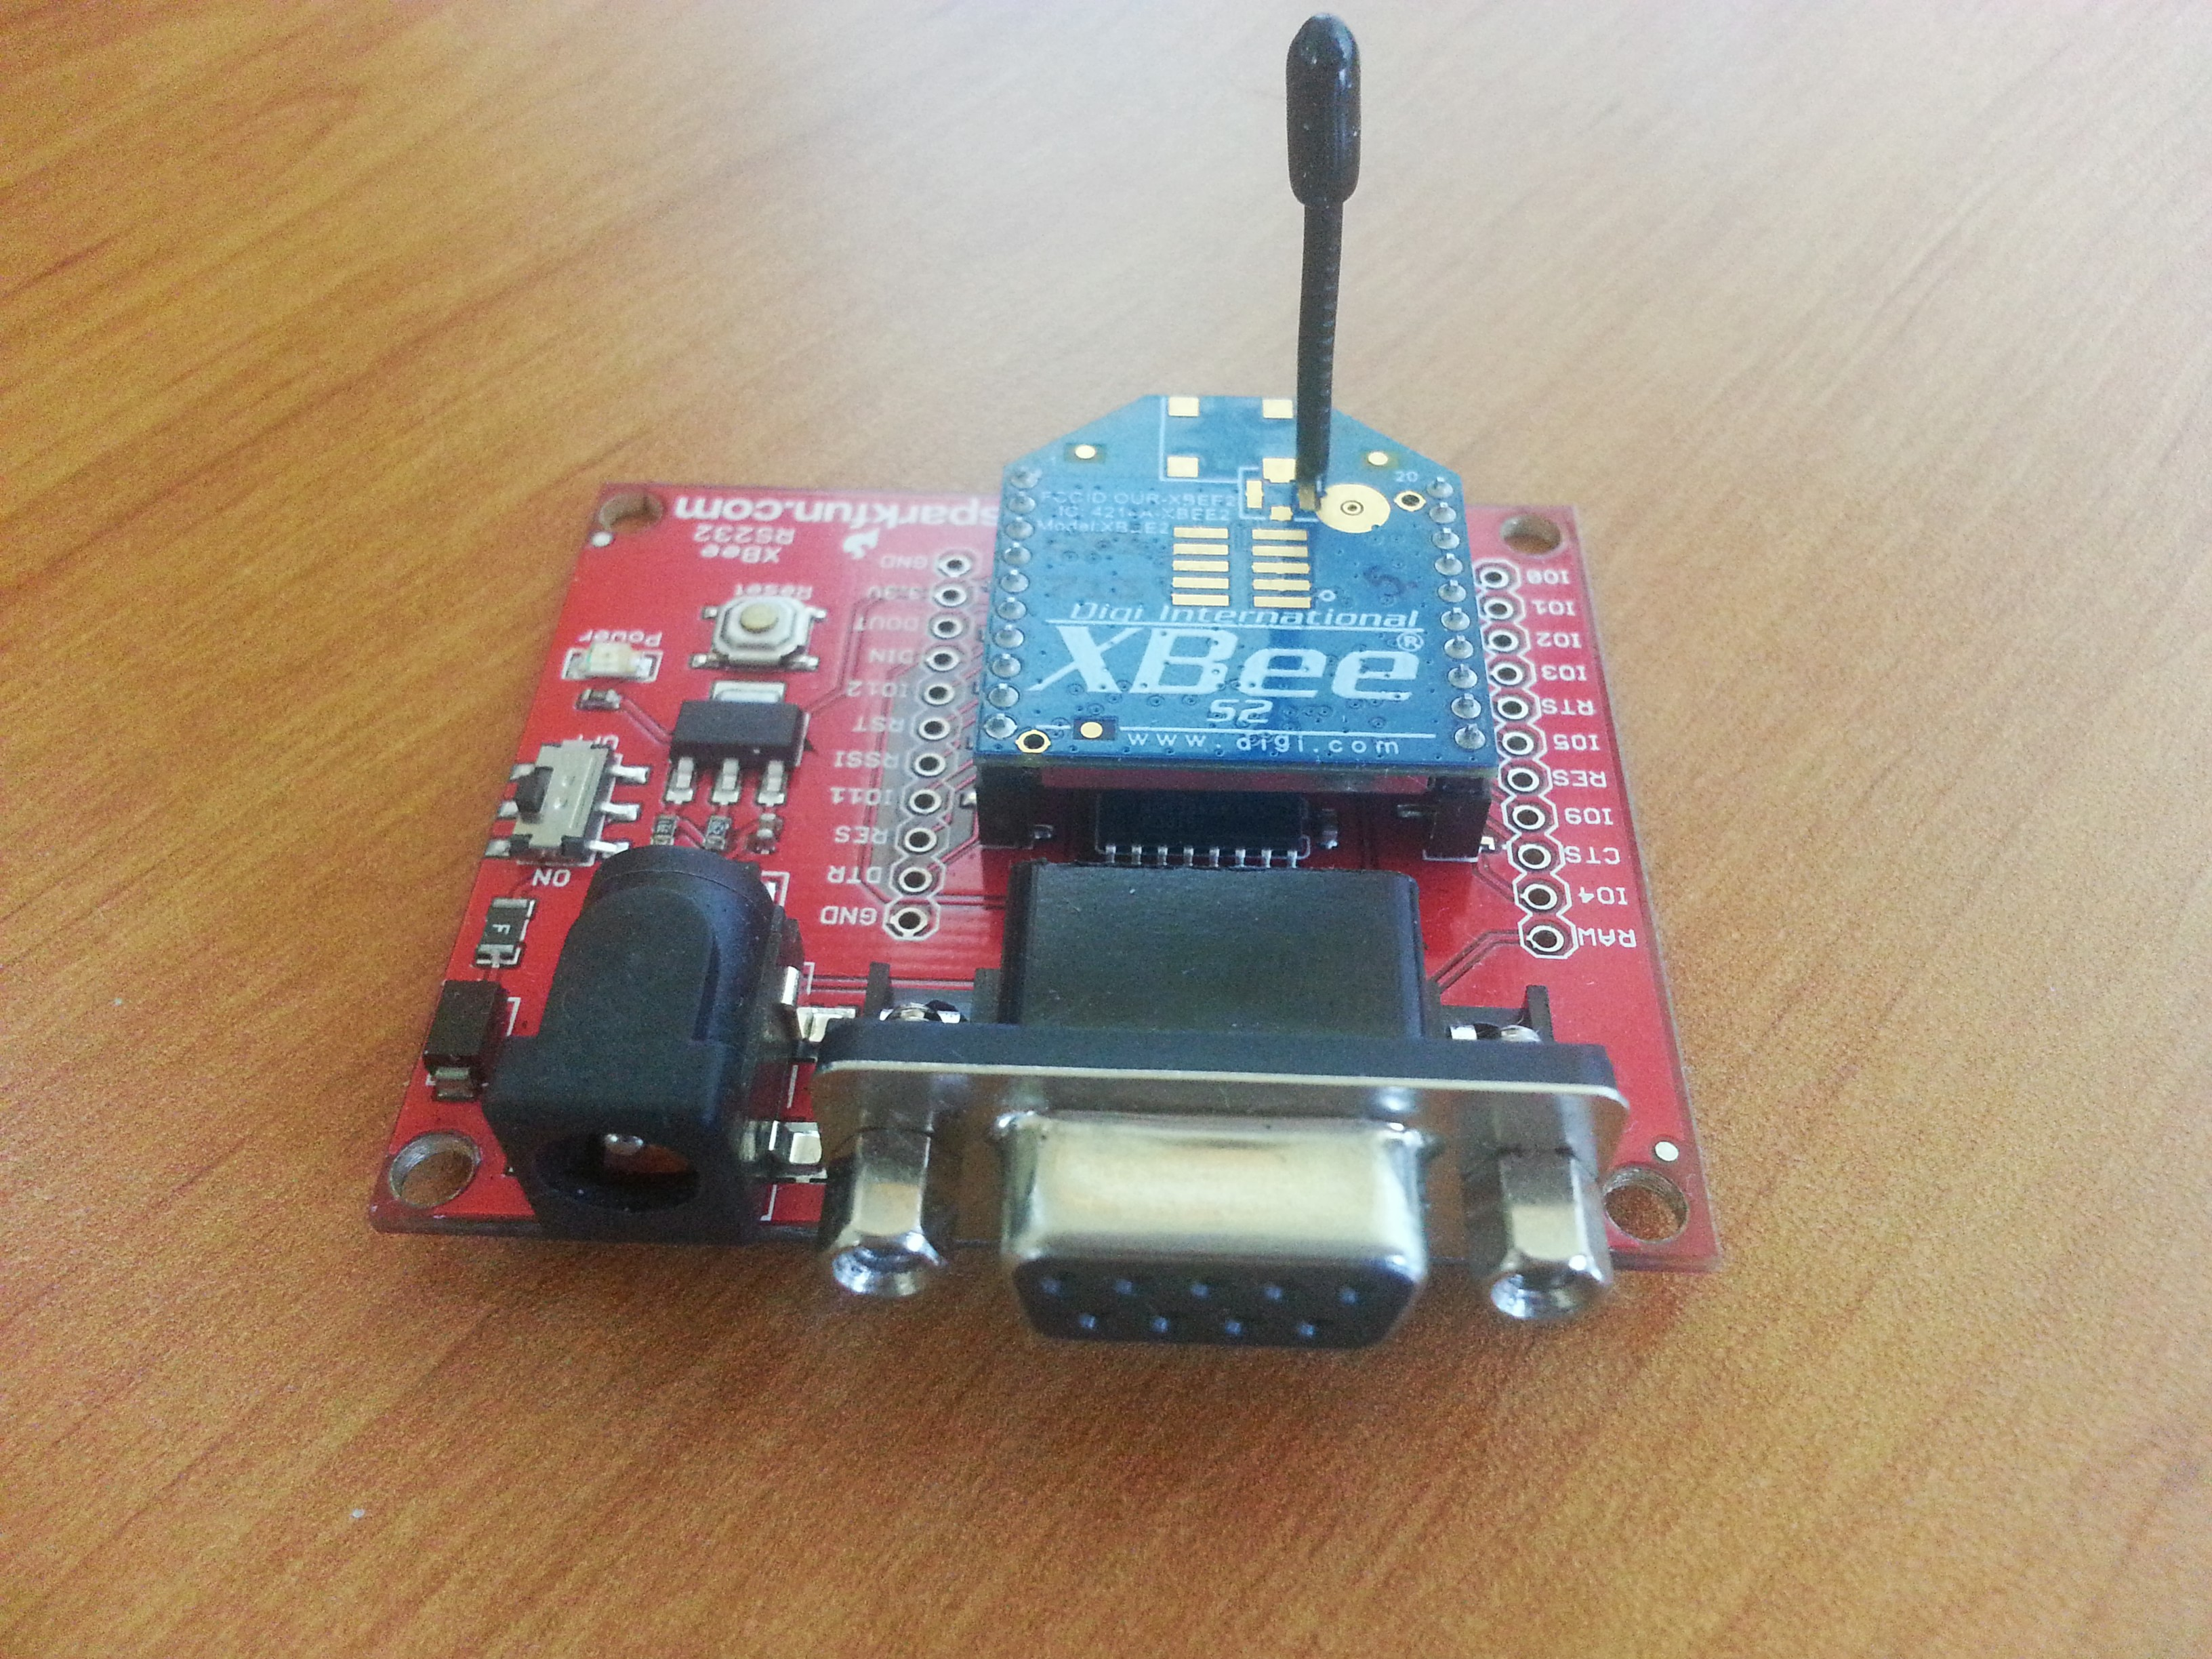
\includegraphics[width=\linewidth*2/3]{img/xbee.jpg}
    \caption{Un module XBEE connecté sur une plaquette de développement}
\end{figure}

\begin{figure}[h!]
    \centering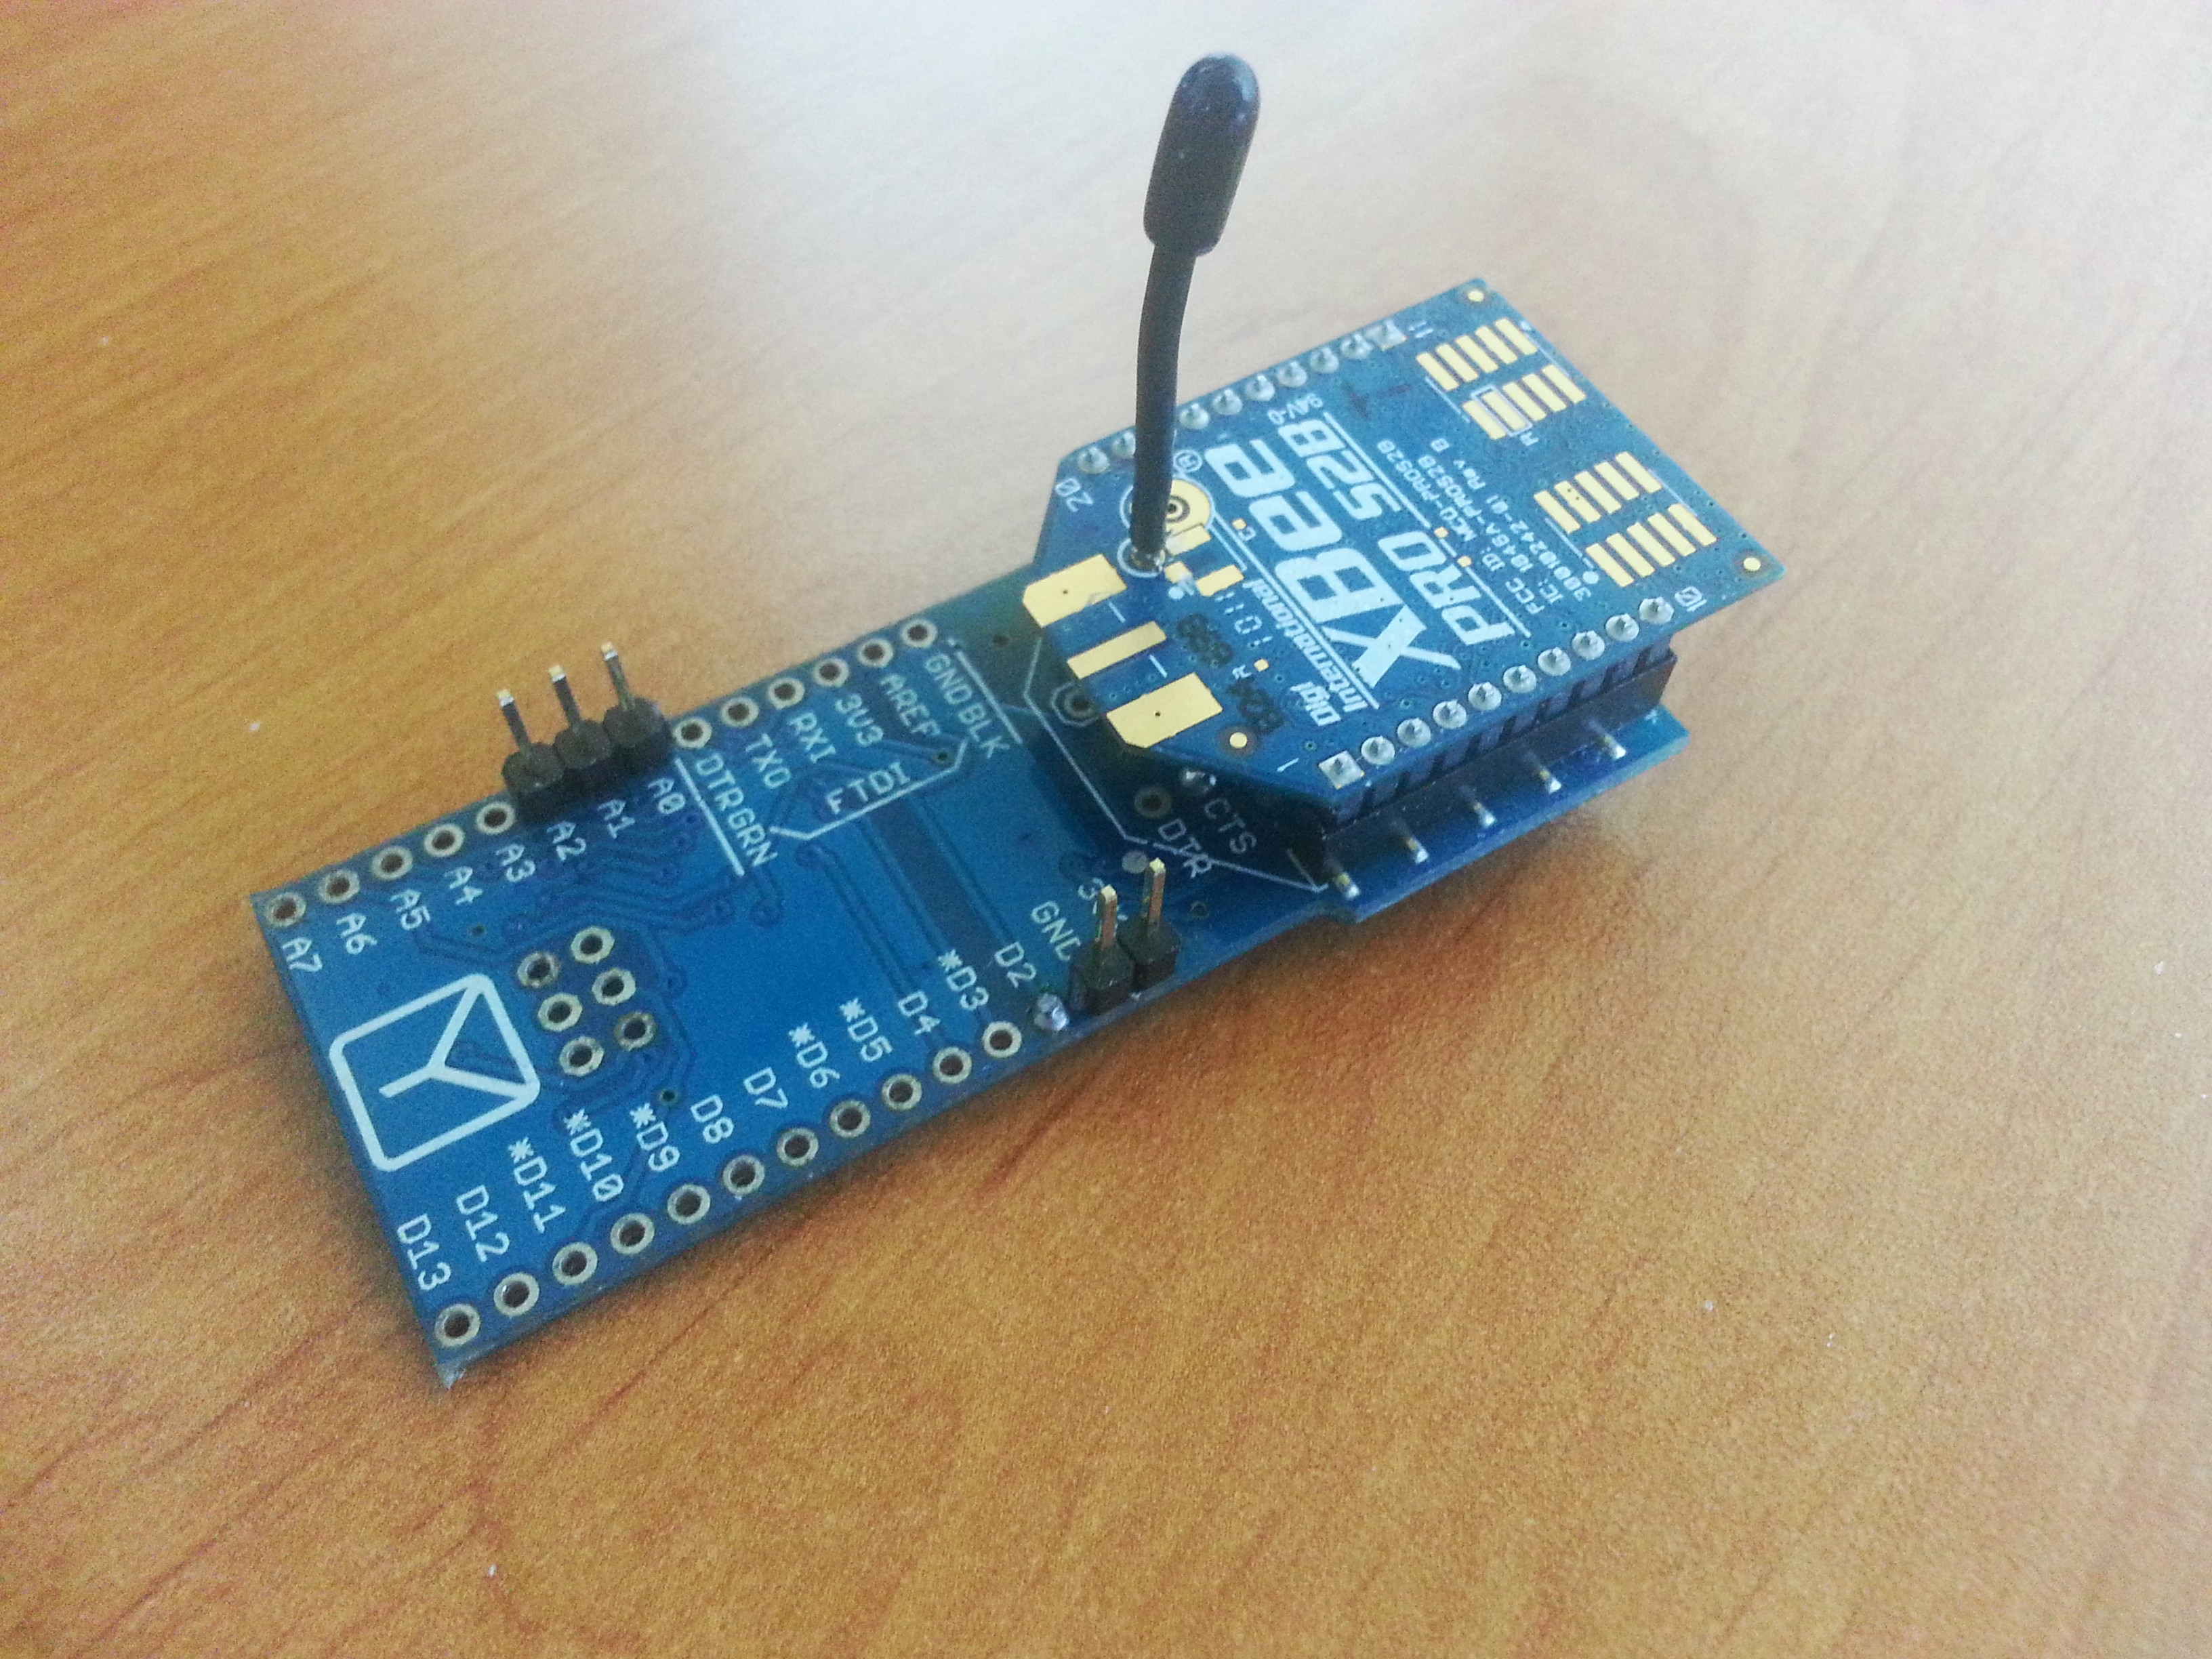
\includegraphics[width=\linewidth*2/3]{img/xbee_2.jpg}
    \caption{Un module XBEE connecté sur un PCB incluant un microcontrolleur}
\end{figure}

\clearpage

\section{Glossaire}
\label{glossaire}

\begin{description}
    \item[Arduino] Voir la \hyperref[arduino]{section Arduino}.
    \item[API] interface de programmation applicative, qui permet à un logiciel de s’interfacer facilement avec d’autres, selon un protocole documenté.
    \item[BeagleBone / BeagleBone Black] Voir la \hyperref[bbb]{section BeagleBone}.
    \item[Callback] fonction de rappel qui est passée en argument à une autre fonction. Cette dernière peut alors en faire usage comme de n'importe quelle autre fonction, alors qu'elle ne la connaît pas par avance.
    \item[Cloud] ensemble de serveurs et d’applications connectés, similaires à un serveur centralisé mais répartis géographiquement et plus puissants.
    \item[CMake] «moteur de production» multi-plateforme. Il sert principalement à simplifier et globaliser la compilation d’un logiciel hétérogène sur diverses plateforme.
    \item[CMS] Composant Monté en Surface, par oposition à des composants électroniques traversants.
    \item[CPack] sous-programme de CMake servant à générer des paquets d’installation pour les distributions Linux.
    \item[Dev Kit] Kit de développement.
    \item[Eclo] Voir la \hyperref[eclo]{section eclo}
    \item[Eclipse (Fondation)] organisme à but non lucratif servant de cadre à un grand nombre de projets logiciels (et principalement l’IDE éponyme). Il fédère entre autres IBM, Oracle, Nokia, Google,…
    \item[Eclipse (IDE)] célèbre Environnement de Développement Intégré en JAVA de la fondation Eclipse.
    \item[EAGLE] Easily Applicable Graphical Layout Editor est un logiciel propriétaire et multi-plateforme de conception assistée par ordinateur de circuits imprimés, comprennant un éditeur de schémas, un logiciel de routage de circuit imprimé, et un éditeur de bibliothèques.
    \item[IDE] Environnement de Développement Intégré: logiciel intégrant entre autres un éditeur de texte, des raccourcis pour utiliser un compilateur, un débugueur, un gestionnaire de versions, …
    \item[IoT] Intenet of Things: ensemble d’objets intelligents connectés internet.
    \item[JSON] JavaScript Object Notation: format de sérialisation en texte simple organisé par paire de clefs/valeurs, où les valeurs peuvent être des nombres, des chaînes de charactère, des listes, ou des dictionnaires.
    \item[LUA] Langage de script libre, réflexif et impératif. Il est proche du Python dans sa syntaxe, mais présente une empreinte mémoire très petite, ce qui lui permet d’être intégré dans un grand nombre de systèmes embarqués, mais aussi de logiciels plus conséquents qui ont besoin d’être scriptable, comme des jeux vidéos.
    \item[M2M] Mobile to Mobile: objets intelligents connectés entre eux à travers internet.
    \item[M3DA] protocole réseau conçu pour un environnement ou le transfert de données est extrêmement couteux.
    \item[Message Queuing] famille de protocoles réseaux fonctionnant sur un principe de messages publiés sur des sujets. Un serveur reçoit les messages publiés par les clients et les publie à son tour à tous les clients qui sont abonnés au sujet.
    \item[mbed] Voir la \hyperref[mbed]{section mbed}
    \item[MQTT] Message Queuing Telemetry Transport: protocole réseau fondé sur un principe de Message Queuing, où l’accent est porté sur la légèreté des données échangées.
    \item[OASIS] Organization for the Advancement of Structured Information Standards: un consortium mondial qui travaille pour la standardisation de formats de fichiers ouverts.
    \item[OEM] Original Equipment Manufacturer: désigne généralement des fabricants de pièces détachées.
    \item[Open-Source / Open-Hardware] Désigne des projets logiciels et/ou matériels dont les codes sources des programmes et/ou les plans de construction du matériel sont disponible librement (et généralement gratuitement). Ce principe permet aux gens de vérifier eux-même leurs logciels/matériels afin de vérifier qu’il se comporte comme prévu, et éventuellement de le modifier si l’on a envie qu’il se comporte différement, de corriger d’éventuels bugs, etc. Pour plus d’informations, voir le site web de la \hyperref[https://www.fsf.org/]{Free Software Foundation}, et \hyperref[freedom defined]{http://freedomdefined.org/OSHW}.
    \item[Open-space] organisation d’un espace de travail où les bureaux sont dans une seule grande pièce.
    \item[Raspberry Pi] Voir la \hyperref[rpi]{section Rasberry Pi}
    \item[REST] style d’architecture utilisant les requettes HTTP pour exposer des API.
    \item[Systemd] remplaçant de SysV fondé sur des programmes binaires plutôt que des scripts shell pour améliorer les performances.
    \item[Socket] en électronique, ce terme désigne une prise femelle spécifique à une puce.
    \item[SMD] Voir CMS
    \item[SysV] premier programme lancé au démarrage de la plupart des distributions GNU/Linux, il s’occupe de lancer les autres.
    \item[Thread] ensemble cohérent de commandes informatiques, pouvant par exemple être éxécuté en parallèle d’un autre Thread.
    \item[Xbee] Voir la \hyperref[xbee]{section Xbee}
    \item[ZigBee] Protocole de communication sans fils maillé à bas prix, concurent du BlueTooth (moins cher, moins complexe et plus fiable dans un grand nombre d’applications), opérant dans la bande 868MHz.
\end{description}

\clearpage


\end{document}
